\documentclass[12pt]{report}
\usepackage{utdiss}
% Imports ---------------------------------------------------------------------

% Required packages.
\usepackage{amsfonts}               % Write mathematics.
\usepackage{amscd}                  % Write mathematics.
\usepackage{amsmath}                % Write mathematics.
\usepackage{amsthm}                 % Write mathematics.
\usepackage{graphicx}               % Include figures from external files.
\usepackage{lmodern}                % Handle font sizes.
\usepackage{makeidx}                % For making an index.
\usepackage{hyperref}               % Embed hyperlinks in the PDF.
\usepackage[nameinlink]{cleveref}   % Make references with \cref{}.
% NOTE: hyperref must be imported BEFORE cleveref.

% Optional packages.
% \usepackage{draftwatermark}       % "DRAFT" watermark in background.

% Packages used solely for the explanation in the template.
\usepackage{layout}                 % Draw the page layout with \layout*.
\usepackage{url}                    % Typesetting URLs.
\usepackage{verbatim}               % Quote block of text verbatim.

% Hyperlink setup -------------------------------------------------------------

\hypersetup{colorlinks=true,allcolors=black}

% Page setup ------------------------------------------------------------------

%% Line spacing (uncomment one).
% \singlespacing \singlespacequote
% \oneandonehalfspacing \oneandonehalfspacequote        % DEFAULT
% \doublespacing \doublespacequote

% Math environments -----------------------------------------------------------

\theoremstyle{plain}        % If changed, also change line 280 of utdiss.sty.
\newtheorem{theorem}{Theorem}[chapter]                  % Number by chapter
\newtheorem{corollary}[theorem]{Corollary}
\newtheorem{lemma}[theorem]{Lemma}
\newtheorem{proposition}[theorem]{Proposition}

\theoremstyle{definition}
\newtheorem{definition}[theorem]{Definition}

\theoremstyle{remark}
\newtheorem{remark}[theorem]{Remark}
\newtheorem*{notation}{Notation}

% Number equations by chapter (Theorem 2.1, 2.2, ...).
\numberwithin{equation}{chapter}
\crefformat{equation}{#2(#1)#3}

% Other customizations --------------------------------------------------------
\usepackage{amssymb,latexsym,amsfonts,amsmath,amsthm, }
\usepackage{graphicx}
\numberwithin{equation}{section}
\newtheorem{example}[theorem]{Example}
\usepackage{minted}
\usepackage[T1]{fontenc}
\usepackage{float}
\usepackage{algorithm}
\usepackage{algorithmic}

\usepackage{minted}
\usepackage{bm}
\usepackage{hyperref}
\usepackage{listings}
\usepackage{xcolor}
\usepackage{soul}

\definecolor{codegreen}{rgb}{0,0.6,0}
\definecolor{codegray}{rgb}{0.5,0.5,0.5}
\definecolor{codepurple}{rgb}{0.58,0,0.82}
\definecolor{backcolour}{rgb}{0.95,0.95,0.92}

\lstdefinestyle{mystyle}{
    backgroundcolor=\color{backcolour},   
    commentstyle=\color{codegreen},
    keywordstyle=\color{magenta},
    numberstyle=\tiny\color{codegray},
    stringstyle=\color{codepurple},
    basicstyle=\ttfamily\footnotesize,
    breakatwhitespace=false,         
    breaklines=true,                 
    captionpos=b,                    
    keepspaces=true,                 
    numbers=left,                    
    numbersep=2pt,                  
    showspaces=false,                
    showstringspaces=false,
    showtabs=false,                  
    tabsize=1
}

\lstset{style=mystyle}


% Author information ==========================================================
\author{Karan Prakash Hiranandani}                        % Author's full name.
\address{karan.hiranandani@utexas.edu}                    % Author's email address.
\title{hIPPYfire:(yet-to-be-finalized)}      % Title of the report.

\supervisor{Dr. Omar Ghattas}

\committeemembers
    {Dr. Umberto Villa, Co-Supervisor}                       % Note the curly braces!

\previousdegrees{B.S}
    % The abbreviated form of your previous degree(s).
    % E.g., \previousdegrees{B.S., MBA}.
    % Default: `B.S., M.S.'
\graduationmonth{May}
     % Graduation month, either May, August, or December, in the form
     % as `\graduationmonth{May}'. Do not abbreviate.
\graduationyear{2023}
     % Graduation year, in the form as `\graduationyear{2001}'.
     % Use the full four-digit number.
\typist{the author}
     % The name(s) of typist(s), put `the author' if you do it yourself.
     % E.g., `\typist{Maryann Hersey and the author}'.

% MASTERS DEGREES ONLY vvvvvvvvvvvvvvvvvvvvvvvvvvvvvvvvvvvvvvvvvvvvvvvvvvvvvvvv

\degree{MASTER OF SCIENCE}            % Or MASTER OF ARTS, for example.
\degreeabbr{M.S.}                     % Or M.A., for example.
% \masterthesis                         % Uncomment ONE of these.
\masterreport                         % Uncomment ONE of these.

% MASTERS DEGREES ONLY ^^^^^^^^^^^^^^^^^^^^^^^^^^^^^^^^^^^^^^^^^^^^^^^^^^^^^^^^

\makeindex

\begin{document} % ============================================================

\copyrightpage

% DOCTORAL DEGREES: committee certification page first, title page second.
\commcertpage
\titlepage

% MASTERS DEGREES: title page first, committee certification page second.
% \titlepage
% \commcertpage

% \begin{dedication} % ----------------------------------------------------------
% A short dedication to someone special.
% \end{dedication}

\begin{acknowledgments} % -----------------------------------------------------
Acknowledgments are technically optional, but come on, it takes a village. Say thanks!
\index{Acknowledgments@\emph{Acknowledgments}}
This section is not limited to a single page.

This \LaTeX{} template was originally written in 1991 by Young~U.~Ryu and later modified by Miguel~A.~Lerma and Craig~McCluskey.
Thanks you guys, we all owe you.
The template was heavily modified by Shane~A.~McQuarrie in 2023.
\index{template!history of}

\end{acknowledgments}

\utabstract % -----------------------------------------------------------------
\indent
\index{Abstract@\emph{Abstract}}
This study presents the implementation of \texttt{hIPPYfire}, a solver for large-scale Bayesian and deterministic inverse problems governed by partial differential equations (PDEs) with infinite-dimensional parameter fields that become high-dimensional after discretization. It utilizes the same scalable algorithms introduced by its predecessor, \texttt{hIPPYlib}, such as the inexact Newton Conjugate Gradient (Newton-CG) method for the computation of the maximum \textit{aposteriori} distribution (MAP point) and the low rank-approximation of the Hessian. These algorithms exploit the fact that several PDE models of physical systems have a low-dimensional solution manifold. \texttt{hIPPYfire} computes the solution of the inverse problem at a cost independent of the parameter dimension, which is measured in terms of the number of linear forward PDE solves. However, unlike \texttt{hIPPYlib} (which is built on FEniCS), \texttt{hIPPYfire} uses Firedrake to solve the PDE governing the forward problem. Firedrake presents a unique modular structure that clearly distinguishes between the programming and mathematical aspects of the library---thereby enabling contributions from programmers and mathematicians alike and ensuring its consistent development. The functionality of the solver is validated by running it on an inverse problem that is governed by an elliptic PDE according to the Bayesian framework. The major components of the inverse problem, namely the forward problem, misfit, and prior functionals, are clearly defined and used to compute the solution of the forward problem and calculate the MAP point using the inexact Newton-CG method. The succesful computation of the forward problem solution and MAP point, coupled with the efficient abstraction in Firedrake, provide motivation to incorporate functionality into \texttt{hIPPYfire}, such as the low-rank approximations of the posterior covariance and the Hessian of the data misfit.


% -----------------------------------------------------------------------------

% \longtocentry                          % Uncomment if using >10 sections.
\tableofcontents
% \listoftables
\listoffigures

% CHAPTERS --------------------------------------------------------------------
\chapter{Intrduction}
\label{chapter:introduction}

The advances made in the fields of high-performance computing have facilitated the development of large-scale solvers for \textit{forward problems}. In a forward problem, inputs (such as the initial and boundary conditions, geometry, sources, material properties etc.) are supplied to the model of a physical system. The forward problem is then solved to determine the output quantities that are of interest. The ready availability of computational resources and the development of powerful discretization techniques that cater to a large variety of models have made the solutions of these forward problems extremely scalable. The vast amounts of data that are available, along with the subsequent improvements in data analysis techniques, have generated commensurate interest in extracting information about the physical model from the observed data. While this progress has been driven by machine learning algorithms, the estimation of physics-based models from data has been a crucial aspect of applied mathematics. Although significant research has already been conducted in this field \cite{banks2012estimation, sullivan2015introduction}, the solution of inverse problems presents a different set of challenges.

Most PDE models of physical systems are characterized by a low-dimensional solution manifold. The inputs to these physical systems include initial and boundary conditions, geometry, sources, material and system properties, etc. The outputs, which are functions of some state variables, are obtained by solving the governing PDEs of the system. The low dimensionality of the map is attributed to the fact that the inputs and outputs are infinite-dimensional (or high-dimensional after discretization). The map from the inputs to the outputs must thus be smoothing, otherwise it may result in information loss. Inverse problems, on the other hand, involve estimation of inputs (commonly known as parameters) from noisy observations of a particular physical model (data). This low-dimensionality of the map causes the estimation of the parameters to be unstable in the presence of noise, which may be present in the system due to the observation process and/or model uncertainty. As a result, the problem is termed to be \textit{ill-posed} due to the violation of one of the three conditions for well-posedness postulated by Hadamard \cite{hadamard1923lectures}. This implies that despite the high-dimensional nature of the data, it does not provide sufficient information to compute a unique solution for the parameter. A computational framework capable of solving such inverse problems, thus, became an important requirement.

This requirement was addressed by \texttt{hIPPYlib}, an inverse problem library that was capable of solving ill-posed large-scale deterministic and Bayesian inverse problems \cite{villa2018hippylib}. \texttt{hIPPYlib} poses the learning-from-data problem as an inverse problem governed by the forward PDE problem. It exploited the low-dimensionality of the parameter-to-observable map to estimate the components of the model at a cost that is measured in terms of the number of forward model solutions. \texttt{hIPPYlib} discretizes the forward map (which is one of the three components of an inverse problem, as discussed in Section \ref{chapter: inverse-problems}) by using the functionality of the \texttt{FEniCS} library---a finite element library for partial differential equations (PDEs) \cite{alnaes2015fenics}. Since the data structures used in the FEniCS library are wrappers on the PETSc library's data structures, \texttt{hIPPYlib} uses PETSC \cite{balay2001petsc} for its linear solvers and algebra operations. The \texttt{FEniCS} library contains different components with multiple layers of abstraction for ease of development and usage. However, given the mathematically complex nature of finite element problems, the consistent development of the FEniCS library and subsequently, that of \texttt{hIPPYlib}, requires individuals highly skilled in programming and FEM concepts.

Similar to the FEniCS project's DOLFIN library \cite{alnaes2015fenics, logg2010dolfin}, Firedrake \cite{rathgeber2016firedrake} is a library that provides automated solutions of partial differential equations (PDEs) using the finite element method (FEM). Firedrake managed to address the abovementioned problems by introducing a new layer of abstraction named PyOP2 \cite{rathgeber2012pyop2}, while maintaining compatibility with FEniCS through the Unified Form Language (UFL) \cite{alnaes2014unified}. The FEniCS Project developed UFL \cite{alnaes2014unified} to express PDEs in a high-level mathematical language and seamlessly integrated it with their DOLFIN library. Well-defined domain-specific languages (DSLs) allow mathematicians to express their problem unambiguously, and Firedrake allows users to express finite element equations in the same syntax as that used in DOLFIN \cite{logg2010dolfin}. UFL is a symbolic language with well-defined finite element semantics, and its integration with Firedrake ensures that users of FEniCS can also use Firedrake with ease.  

Thus, the need for an inverse problem library built on a modularized FEM solver like Firedrake led to the conception of \texttt{hIPPYfire}. This study presents the structure and implementation of \texttt{hIPPYfire}---an inverse problem library modelled similar to \texttt{hIPPYlib}, but built on Firedrake. The algorithms implemented in \texttt{hIPPYfire} are identical to those implemented in \texttt{hIPPYlib}. However, there are minor differences in the utilities and linear algebra functions due to the currently limited functionality of the Firedrake library---all of which have been elaborated and expanded upon in the following sections of this report.

Section \ref{chapter: inverse-problems} provides a brief introduction to the theory behind inverse problems. The advantages of the Firedrake library over FEniCS are explained with some technical context in Section \ref{chapter: software}. Emphasis is also placed on the shortcomings of the Firedrake library and the development of custom linear algebra methods to address them. The structure of \texttt{hIPPYfire} is also discussed in Section \ref{chapter: software}. The \texttt{hIPPYfire} library is validated in Section \ref{chapter:sample-problem} by creating a test case involving a Bayesian inverse problem. This section is followed by the conclusion (Section \ref{chapter:conclusion}), which discusses the development roadmap for \texttt{hIPPYfire}.
\chapter{Theory Behind Inverse Problems}
\label{chapter: inverse-problems}
This section discusses two general approaches adopted to solve inverse problems---namely the determinstic framework \cite{laloy2019gradient, vogel2002deterministic} and Bayesian framework \cite{dashti2017bayesian, stuart2010inverse} for inverse problems. \texttt{hIPPYfire} currently implements an infinite-dimensional Bayesian framework \cite{thanh2013infinitebayesian}, and consequently, additional emphasis has been placed on the theory of the latter framework.

Lower-case italic font is used to represent scalar valued functions like the parameter \textit{m}, state \textit{u}, observed data \textit{d} etc. The discretized equivalents of these functions $\mathbb{R}^n$ (where \textit{n} is the discretization dimension) are denoted with a bold, lowercase font, such as \textbf{m}, \textbf{u}, \textbf{d} etc. Vector functions in $\mathbb{R}^2$ or $\mathbb{R}^3$ are denoted in italic, bold, lowercase font, such as \textbf{\textit{v}} (velocity field). Infinite-dimensional spaces are represented through calligraphic font, such as $\mathcal{A}$. Scalars are denoted by using Greek font.


\section{Deterministic Inversion}
\label{sec:det_inversion}

The solution of an inverse problem involves the inference of the parameter \textit{m} $\in \mathcal{X}$, given data \textit{\textbf{d}} $ \in \mathbb{R}^q$ by using the following \textit{parameter-to-observable} map:
\begin{equation}
\label{eqn:fwd_map}
    \mathcal{F}(m) = d + \eta
\end{equation}

Similar to \textit{hIPPYlib}, the linear or non-linear \textit{parameter-to-observable (p2o)} map is depicted as $\mathcal{F} : \mathcal{M} \rightarrow \mathbb{R}^q$. Note that $\mathcal{M} \subseteq L^2(\mathcal{D})$, where $\mathcal{D} \subset \mathbb{R}^d$ is a bounded domain.  It is important to distinguish between the \textit{p2o} map the forward problem. The forward problem is a map from the parameter \textit{m} to the PDEs that govern the physical system, i.e., $m \rightarrow r(u, m)$, where $r(u, m)$ is the residual and \textit{u} $\in \mathcal{V}$ is a state variable and $\mathcal{V}$ is a Hilbert Space of functions defined on $\mathcal{V}$.

The forward problem is one of the three components of the forward map $\mathcal{F}$. The second component is the map $r: \mathcal{V} \times \mathcal{M} \rightarrow \mathcal{V}^*$. This map involves the solution of the governing PDEs. The third component is the observation operator $\mathcal(B)$, which maps \textit{u} to the observable \textit{y} $\in \mathbb{R}^q$, which can be high or infinite dimensional. Thus, the map $\mathcal{F}$ is now defined as:
\begin{equation}
    \mathcal{F}(m) = \mathcal{B}(u), given, r(u, m) = 0
\end{equation}
The noise, $\eta$, accounts for the difference between the observable \textit{y} and data \textit{\textbf{d}} and is modelled as a Gaussian centred at 0 with a covariance $\Gamma_{noise}$. The source of the noise can be traced to imprecise measurements, model, and/or numerical errors. Although their exact values are not known, their statistical information (mean, variance, etc.), are known.

The ill-posedness of inverse problems \cite{tikhonov1963solution}, as discussed earlier, can primarily be attributed to their instability. The collapse of the spectrum of $\mathcal{F}$ is the main culprit behind this phenomenon. The small eigenvalues of $\mathcal{F}$, which correspond to eigen function modes below the noise threshold, cause the noise in the data to blow up exponentially---rendering the inversion useless. The most obvious solution to this problem would be to discard the irrelevant eigenvalues. Although a truncated SVD presents a viable solution to the problem, the \textit{Tikhonov Regularization} technique \cite{golub1999tikhonov} allows us to formulate the inverse problem as an optimization problem instead of applying a filter. This can be mathematically represented as a non-linear least squares optimization problem:
\begin{equation}
\label{eqn:deterministic2}
    \underset{m \in \mathcal{M}}{min}\mathcal{J}(m) := \frac{1}{2} ||\mathcal{F}(m) - \textbf{\textit{d}} ||^2_{\Gamma^{-1}_{noise}} + \mathcal{R}(m)
\end{equation}
$\mathcal{J}(m)$ represents the cost functional. The first term on the RHS represents the misfit between $\mathcal{F}(m)$, weighted by the inverse noise covariance $\eta^{-1}_{noise}$, and data \textit{\textbf{d}}. The regularization parameter, $\mathcal{R}(m)$, ensures smoothness on the inversion parameter \textit{m}.

Information on the first and second derivatives (gradient and Hessian, respectively) is required to solve the nonlinear optimization problem. Lagrangian techniques \cite{troltzsch2010optimal} were adopted in the development of the \texttt{hIPPYlib} library \cite{villa2018hippylib} to compute the actions of the Hessian and gradient. \texttt{hIPPYfire} makes use of the \textit{Inexact Newton Conjugate Gradient Method} to solve the optimization problem, similar to the flow followed by \texttt{hIPPYlib} \cite{villa2018hippylib}.

The regularization technique of solving inverse problems \eqref{eqn:fwd_map}, although scalable with efficient inverse solvers, fails to account for uncertainties in the inferred parameters. This can be attributed to the fact that this approach only provides a point estimate of the inverse problem. Thus, it is not very useful for ill-posed problems with non-negligible noise---thereby prompting the conception of the Bayesian framework.

\section{Bayesian Inversion}
\label{sec:bayesian_inversion}
The Bayesian framework treats the inverse problem as statistical inference over a space of uncertain parameters. It computes a \textit{posterior probability distribution} which represents the probability of the parameter being conditioned on the given data. One of the components of this framework is a \textit{prior distribution}, which accounts for any constraints or assumptions on the data before data collection. This is combined with the \textit{likelihood}, which expresses the probability of obtaining the observed data from a given set of parameters. This is achieved by analyzing and characterizing the posterior through mean estimation, sample drawing, analysis of the covariance etc.

However, complete characterization of the posterior is impractical for expensive PDE forward models, especially for ones in high dimensions that have been obtained after the discretization of infinite-dimensional parameter fields. Recently developed techniques, however, take advantage of the low dimensionality to address these problems---similar to the properties of the deterministic framework. Some of these include forward model reduction \cite{galbally2010non}, Markov chain Monte-Carlo techniques that utilize the log-likelihood Hessian approximations \cite{petra2012inexact}, randomize-then-optimize techniques \cite{wang2018randomized}, etc. \texttt{hIPPYfire}, much like its predecessor \cite{villa2018hippylib}, uses \textit{Lagrangian approximation} of the posterior. This is extremely scalable and efficient---especially if the same properties that made the regularized Newton-CG method so powerful are used.

The infinite-dimensional Baye's formula is given as:
\begin{equation}
    \label{eqn:posterior}
    \frac{d\mu_{post}}{d\mu_{prior}} \propto \pi_{like}(\textbf{d}|m)
\end{equation}
The LHS and RHS represent the Radon-Nikodym derivative \cite{williams1991probability} and likelihood, respectively. 
To study the impact of the noise on the likelihood, the noise is modelled as a centered Gaussian on $\mathbb{R}^q$ with a covariance of $\Gamma_{noise}$. Thus, the likelihood can be expressed as
\begin{equation}
    \label{eqn:noise-likelihood}
    \pi_{like}(\textbf{d}|m) \propto exp(-\Phi(m))
\end{equation}
where $\Gamma(m) = \frac{1}{2}||\mathcal{F}(m) - \textbf{\textit{d}}||^2_{\Gamma_{noise}^{-1}}$ denotes the negative log-likelihood.
The prior is chosen to be Gaussian, giving the following relation:
\begin{equation}
    \label{eqn:prior}
    d\mu_{prior}(m) \propto exp\{ -\frac{1}{2}|| m - m_{pr} ||^2_{C^{-1}_{prior}} \}
\end{equation}
where $m \sim \mathcal{N}(m_{pr}, C_{prior})$. For a parameter that represents a spatial field on $\mathcal{D} \in \mathbb{R}^d$, the prior covariance operator $C_{prior}$ ensures that the computed parameter is smooth and depends continuously on the data. The motivation behind this is to avoid the presence of discontinuous or rough components in the parameter, which makes it difficult to infer the latter from the data. The construction of the prior is similar to the methodology followed by \texttt{hIPPYlib} \cite{villa2018hippylib}.
The equations of the likelihood (Eqn. \eqref{eqn:noise-likelihood}) and prior (Eqn.\eqref{eqn:prior}) are substituted in the posterior distribution equation (Eqn. \eqref{eqn:posterior}) to yield:
\begin{equation}
    \label{eqn:posterior2}
    d\mu_{post} \propto exp \{ - \frac{1}{2}||\mathcal{F}(m) - \textbf{\textit{d}}||^2_{\Gamma^{-1}_{noise}} - \frac{1}{2}||m - m_{pr}||^2_{C^{-1}_{prior}} \}
\end{equation}

The next step in the flow involves the computation of the MAP point $m_{MAP}$---which is the parameter field that maximizes the posterior distribution. It is obtained by solving the following optimization problem:
\begin{equation}
    \label{eqn:map}
    m_{MAP} := \underset{m \in \mathcal{M}}{argmin}\frac{1}{2}||\mathcal{F}(m) - \textbf{\textit{d}}||^2_{\Gamma_{noise}^{-1}} + \frac{1}{2}||m - m_{pr}||^2_{C_{prior}^{-1}}
\end{equation}

It is noteworthy that the prior performs the role of \textit{Tikhonov Regularization} \cite{golub1999tikhonov}. Similaritires can be drawn between Eqn. \eqref{eqn:map} and Eqn. \eqref{eqn:deterministic2}. In case the \textit{p2o} map is non-linear, the posterior does not follow a Gaussian distribution. However, certain assumptions can be made on the noise covariance $\Gamma_{noise}$, number \textit{q} of observations, and regularity of the \textit{p2o} map $\mathcal{F}$, the Laplace approximation can be utilized to estimate the expected value of the prior \cite{tierney1986accurate, evans2000approximating}. This is followed by the discretization of the Bayesian inverse problem, which has been explained in \cite{thanh2013infinitebayesian, villa2018hippylib}. The complete implementation of the Laplace approximation, along with the Bayesian discretization, in \texttt{hIPPYfire} is similar to that of \texttt{hIPPYlib} \cite{villa2018hippylib}.
\chapter{Software Framework}
\label{chapter: software}

\section{Firedrake}
\label{section:Firedrake}
As mentioned previously, one of the improvements Firedrake \cite{rathgeber2016firedrake} implemented over FEniCS \cite{alnaes2015fenics} is the creation of a new abstraction layer, namely PyOP2 \cite{rathgeber2012pyop2}, to distinguish between the local discretization or mathematical operators and their parallel execution over the mesh in the implementation layer. Firedrake models a finite problem as a combination of several abstractions---thereby allowing the user to follow a modularized approach while defining their problem.
 \begin{figure}[th]
        \centering
        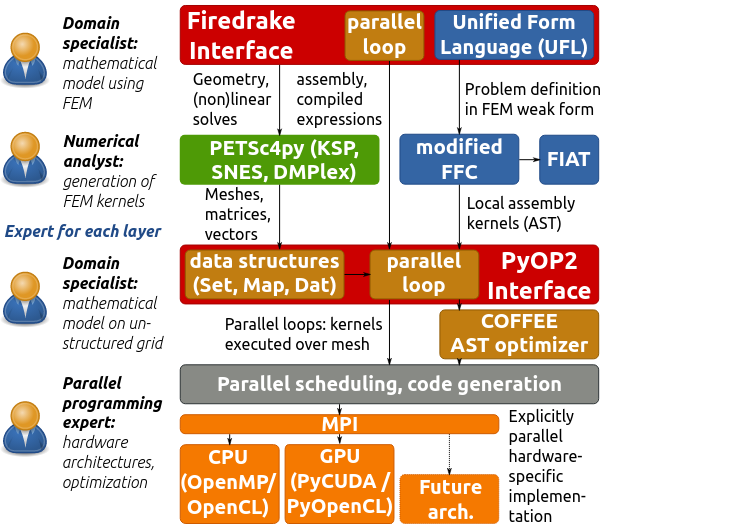
\includegraphics[width=0.8\textwidth]{figures/firedrake_toolchain_users.png}
        \caption{Firedrake Abstractions}Depiction of the separation of user concerns in Firedrake.Tools using FEniCS and PETSc are highlighted in blue and green respectively. The PyOP2 layers are shown in brown, while the backend engine is shown in orange \cite{rathgeber2016firedrake}.
        \label{figure:parameter}
        \end{figure}
As mentioned earlier, Firedrake improved upon FEniCS by adopting a philosophy that emphasized on the separation of concerns---thereby providing a clear distinction between the mathematical and programming aspects of the library. Since a multidisciplinary skillset, which ranges from mathematical expertise in numerical analyses to a deep understanding of parallel computation, is required for the development of these tools, it became more practical to develop abstract layers in the library that catered to a particular skillset. Firedrake introduced a new layer of abstraction named PyOP2 \cite{logg2010dolfin} that clearly formed a distinction between the finite element interface and the parallel execution of its algorithm over the mesh. PyOP2 thus creates a separation between the discretization of the mathematical operators and their parallel execution over the mesh. This has made the Firedrake codebase significantly more compact.  

The cost of typical finite element problems can be attributed to data movement and floating point operations---both of which are proportional to the mesh size. These operations can be divided into two categories---custom mesh-defined data structure iterations and sparse linear algebra. While Firedrake utilizes PETSc \cite{balay2001petsc} for the latter, PyOP2 was designed to address the former \cite{rathgeber2012pyop2}. Additional information regarding the integration of PyOP2 with the Firedrake layer is shown in the figure below \cite{rathgeber2016firedrake}.
\begin{figure}[th]
        \centering
        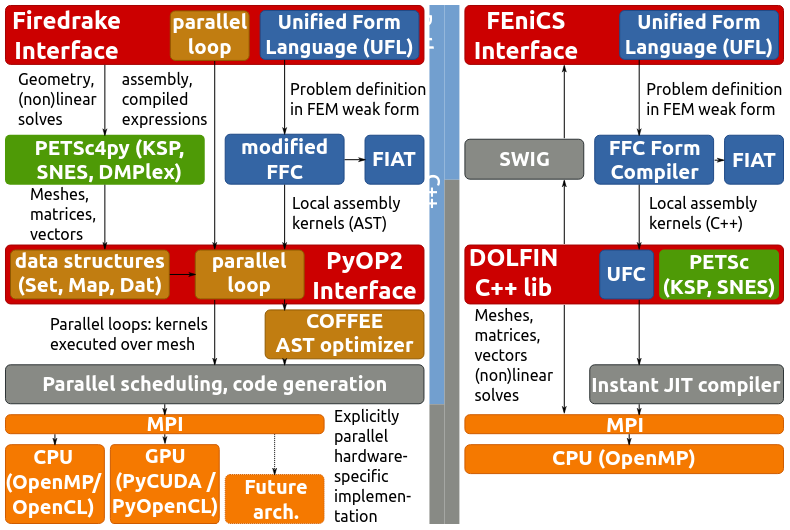
\includegraphics[width=0.8\textwidth]{figures/firedrake_toolchain_dolfin.png}
        \caption{Firedrake v/s FEniCS flow}The clear distinction introduced in Firedrake is evident from the PyOP2 interface in its flow. \cite{rathgeber2014firedrake}.
        \label{figure:parameter}
        \end{figure}

The primary motivation behind using Firedrake can be attributed to its improved abstraction layer. However, a comparative analysis of the performances of Firedrake and FEniCS was conducted \cite{rathgeber2016firedrake}. Firedrake reported a better performance than FEniCS---however, no concrete reason has been provided for its superior performance.


\section{ \texttt{hIPPYfire} }
\label{section:hIPPYfire}
\texttt{hIPPYfire} attempts to accomplish the same objective as that of \texttt{hIPPYlib} , i.e., implementation of scalable algorithms for PDE-based deterministic and Bayesian inverse problems. However, unlike its predecessor, it is built on Firedrake instead of FEniCS. The user is required to provide the PDE problem and likelihood in UFL \cite{alnaes2014unified}, and \texttt{hIPPYfire} computes the gradient and Hessian. \texttt{hIPPYfire} is currently in development and does not support all the functionality of \texttt{hIPPYlib} at the timing of writing this report. Its different components have been summarized below:
\begin{itemize}
    \item \textbf{Models}: The \texttt{modeling} module allows the user to specify information on the forward problem, misfit functional, and the prior. 
    \begin{enumerate}
        \item Forward Problem: This module computes the solutions of the forward, adjoint, and incremental problems. \texttt{hIPPYlib} and \texttt{hIPPYfire} both accept user input for the forward problem as a UFL form or user-defined object. The latter is required for transient inverse problems. However, if the forward problem is input as a UFL form, \texttt{hIPPYfire} computes the gradient and Hessian as well.
        \item Misfit: The misfit module evaluates the negative log-likelihood and its derivatives. Currently, the only misfit functional \texttt{hIPPYfire} provides support for is that of continuous observations---however, other functionals are currently in development.
        \item Prior: The prior computes the negative log-density and its derivatives, in addition to drawing samples and estimating the marginal variance. The user can select a Bilaplacian prior in \texttt{hIPPYfire}'s current implementation. There is a provision to accept user-defined priors as well.
        \item Model: The model is used to set up the \textit{p2o} map. Its three components are computed from the abovementioned modules.
        \item Hessian: If the forward problem is input in a standard UFL form, \texttt{hIPPYfire} internally computes the Hessian of the forward map. The collapse of the spectrum of the Hessian significantly influences the ill-posedness of the problem. However, the Hessian assumes a dense structure after discretization, thereby requiring forward and adjoint solves. Since the dimension of the Hessian is equal to that of the parameter, computing the Hessian for large-scale problems is not feasible. The rapidly decaying spectrum of the Hessian is exploited because the eigenvalues that tend to zero contain minimal information about the infinite-dimensional parameter field \cite{flath2011fast, bui2012analysis}.   
    \end{enumerate}  
    In case of transient problems, the user will have to provide their own derivatives.
    \item \textbf{Algorithms}: The \texttt{algorithms} module contains an implementation of the inexact Newton-CG algorithm \cite{borzi2011computational}. This is used to solve the deterministic inversion problem and compute the maximum \textit{a posteriori} distribution (also called the MAP point) for Bayesian inversion problems. Following the computation of the gradient and Hessian forms, the Newton system is solved according to the Steihaug criterion \cite{steihaug1983local}. Additional information regarding the implementation of this algorithm can be found in Villa et al. \cite{Villa2020}.  Custom linear algebra algorithms have also been implemented to perform basic matrix-vector operations that have been described later in this section.
    \item \textbf{Utilities}: The \texttt{utils} module contains certain helper functions to extract relevant data. The \texttt{vector2function} module wraps a discrete vector onto a continuous function, while the \texttt{rand} module generates random functions that are used to model the noise function and vector. The \texttt{parameterlist} module creates a custom list of parameters for the Newton solver.

    \begin{figure}[th]
        \centering
        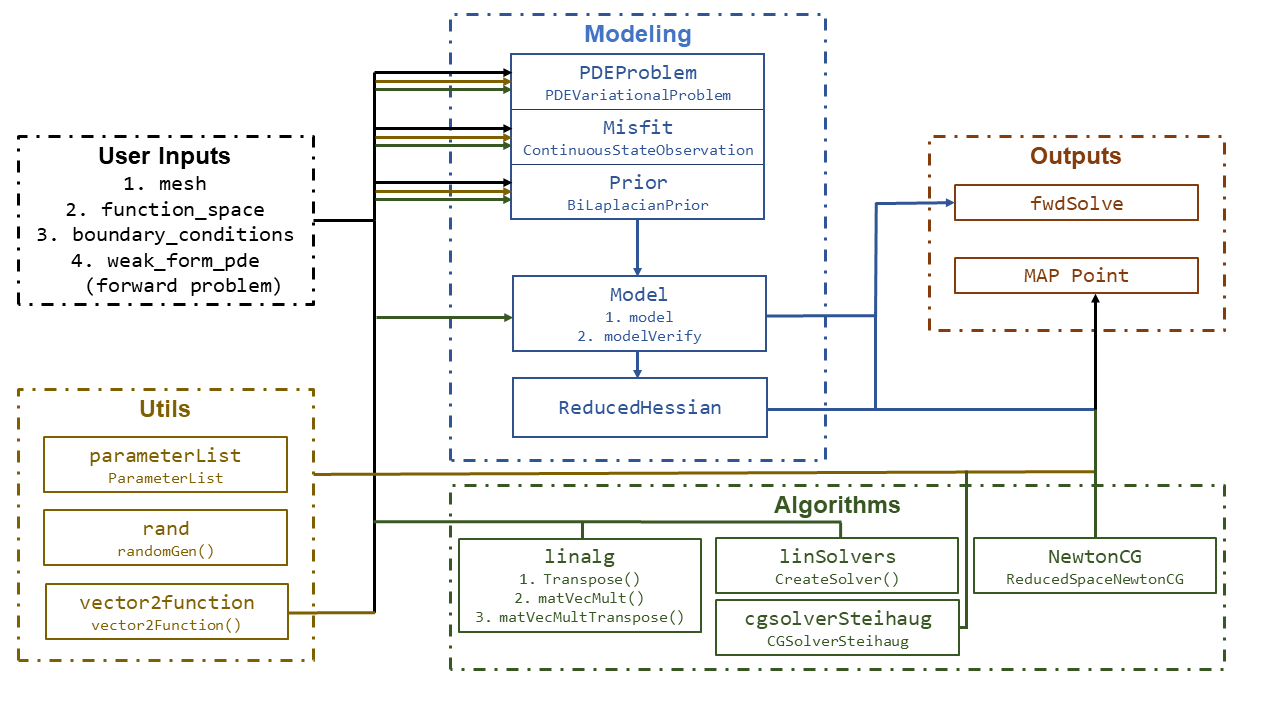
\includegraphics[width=1.0\textwidth]{figures/hIPPYfire.png}
        \caption{Flow and functionality of \texttt{hIPPYfire}}
        \label{figure:hippyfire}
    \end{figure}
    
    One of the major challenges faced in the development of \texttt{hIPPYfire} was the limited functionality of Firedrake's \texttt{firedrake.matrix.Matrix} data structure. Certain modules required matrix transpose and matrix-vector multiplication operations. Since these operations are not defined for the firedrake Matrix, Firedrake's interface with PETSc was used to create linear algebra operations between Firedrake objects and their PETSc wrappers. These operations include matrix transpose (\texttt{Transpose()}, matrix-vector multiplication (\texttt{matVecMult()}), and matrix-transpose-vector multiplication (\texttt{matVecMultTranspose()})---all of which have been defined in the \texttt{linalg} module. 
    The \texttt{hIPPYlib} library provides APIs to create different kinds of solvers (the \texttt{PETScKrylovSolver()} and \texttt{PETScLUSolver()}, \texttt{hIPPYfire} provides a single API (\texttt{CreateSolver()}), which acts as a wrapper for Firedrake's linear solvers API and allows the user to create their custom solver.
\end{itemize}
\chapter{Sample Problem}
\label{chapter:sample-problem}

In order to validate the different modules of \texttt{hIPPYfire}, one of \texttt{hIPPYlib}'s Bayesian inversion test cases, namely \texttt{3-SubsurfaceBayesian} \cite{Villa_hIPPYlib_An_Extensible_2020}, was recreated. This test case utilized all of \texttt{hIPPYfire}'s models that have been currently developed. Additional test cases shall be added for future functionality. The test case is briefly discussed below; a detailed description of the test case can be found in \texttt{hIPPYlib}'s repository \cite{Villa_hIPPYlib_An_Extensible_2020}.

This test case solves the forward problem and computes the MAP point, as described in Section \ref{chapter: inverse-problems}. The forward problem of this test case is governed by an elliptic PDE. The objective is to compute the parameter fields with a certain probability that these gave rise to the observed data. Please note that the following test case admits discretized expressions of the parameter space, i.e., they are finite-dimensional.

A Gaussian prior is assumed with a mean of $\textbf{m}_{prior}$. Its covariance, \textbf{$\Gamma_{prior}$}, is obtained by discretizing the inverse of the differential operator $\mathcal{A}^{-2} = (-\gamma\Delta + \delta\textbf{I})^{-2}$, where $\gamma, \delta > 0 $. The prior is chosen such that the well-posedness of this problem is ensured.

The likelihood is calculated as shown below:
\begin{equation}
    \textbf{d}_{obs} = \textbf{f(m)} + \textbf{e}
\end{equation}
$\textbf{e}$ represents the noise, which is computed by the \texttt{randomGen()} method in the \texttt{rand} module.
\begin{equation}
    \pi_{like}(\textbf{d}_{obs} | \textbf{m}) = exp(-\frac{1}{2}(\textbf{f(m)} -\textbf{d}_{obs})^T\Gamma^{-1}_{noise}(\textbf{f(m)} -\textbf{d}_{obs}))
\end{equation}

The above equation presents a discretized version of the likelihood function. The mean of the posterior distribution, also referred to as \textbf{${m_{MAP}} $}, is the parameter vector that maximizes the posterior. Its discretized computation is listed below:
\begin{equation}
    \textbf{m}_{MAP} := \underset{m}{arg min}\mathcal{J}(\textbf{m}) := (\frac{1}{2} || \textbf{f(m)} - d_{obs} ||^2_{\Gamma_{noise}^{-1}} + \frac{1}{2}|| \textbf{m} - \textbf{m}_{prior} || ^2_{\Gamma_{noise}^{-1}}
\end{equation}

Problem flow has been defined until the computation of the MAP point in \texttt{hIPPYfire}. A few code snippets have been included below

\begin{itemize}
    \item \textbf{Mesh and FEM setup}: A two-dimensional unit square mesh is created with a P2 finite element space for \texttt{state} and \texttt{adjoint} variables and P1 for \texttt{parameter}.
    \begin{lstlisting}[language=python]
        ndim = 2
        nx = 64
        ny = 64
        mesh = fd.UnitSquareMesh(nx, ny)
        Vh2 = fd.FunctionSpace(mesh, 'Lagrange', 2)
        Vh1 = fd.FunctionSpace(mesh, 'Lagrange', 1)
        Vh = [Vh2, Vh1, Vh2]
    \end{lstlisting}
    \item \textbf{Forward Problem}: As mentioned in Section \ref{chapter: software}, the \texttt{PDEVariationalProblem} class sets up the forward problem component of the \textit{p2o} map. In addition to the finite element components defined above, it requires an expression of the weak form of the PDE (given by \texttt{pde\_varf}) and boundary conditions for the forward (\texttt{bc}) and incremental and adjoint problems (\texttt{bc0}).
    The \texttt{PDEVariationalProblem} class solves the forward/adjoint and incremental problems and computes the relevant partial derivatives with respect to the state, parameter, and adjoint variables.
    \begin{lstlisting}[language=python]
        u_bdr = fd.SpatialCoordinate(mesh)[1]
        u_bdr0 = fd.Constant(0.0)

        bc = fd.DirichletBC(Vh[STATE], u_bdr, [3, 4]) # [3, 4] indicates that bc is applied to y == 0 amd y ==1
        bc0 = fd.DirichletBC(Vh[STATE], u_bdr0, [3, 4])

        f = fd.Constant(1.0)

        def pde_varf(u, m, p):
            return ufl.exp(m) * ufl.inner(ufl.grad(u), ufl.grad(p)) * ufl.dx - f * p * ufl.dx

        pde = PDEVariationalProblem(Vh, pde_varf, bc, bc0, is_fwd_linear=True)
    \end{lstlisting}
    The \texttt{is\_fwd\_linear=True} flag allows the user to set a non-linear forward map as well.
    \item \textbf{Prior setup}: The class \texttt{BiLaplacianPrior} creates a Gaussian prior with zero average, Additional information regarding the covariance can be found in Villa et al. \cite{Villa_hIPPYlib_An_Extensible_2020}.
    \begin{lstlisting}[language=python]
        pr = BiLaplacianPrior(Vh[PARAMETER], gamma, delta, robin_bc=True)
        x = fd.SpatialCoordinate(mesh)
        mtrue = fd.interpolate(fd.sin(x[0])*fd.cos(x[1]), Vh[PARAMETER]).vector()
        m0 = fd.interpolate(fd.sin(x[0]), Vh[PARAMETER]).vector()
        objs = [fd.Function(Vh[PARAMETER], mtrue), fd.Function(Vh[PARAMETER], pr.mean)]
    \end{lstlisting}
    The true parameter, \texttt{mtrue} is initialized to be a known analytic function to validate the accuracy of the parameters cmoputed by \texttt{hIPPYfire}. Plots of the vectors \texttt{mtrue} and \texttt{pr.mean} are generated and shown below. For the purpose of validation through this test case, \texttt{mtrue} is a known function and not randomly generated, as in \texttt{hIPPYlib} \cite{Villa_hIPPYlib_An_Extensible_2020}
        \begin{figure}[th]
        \centering
        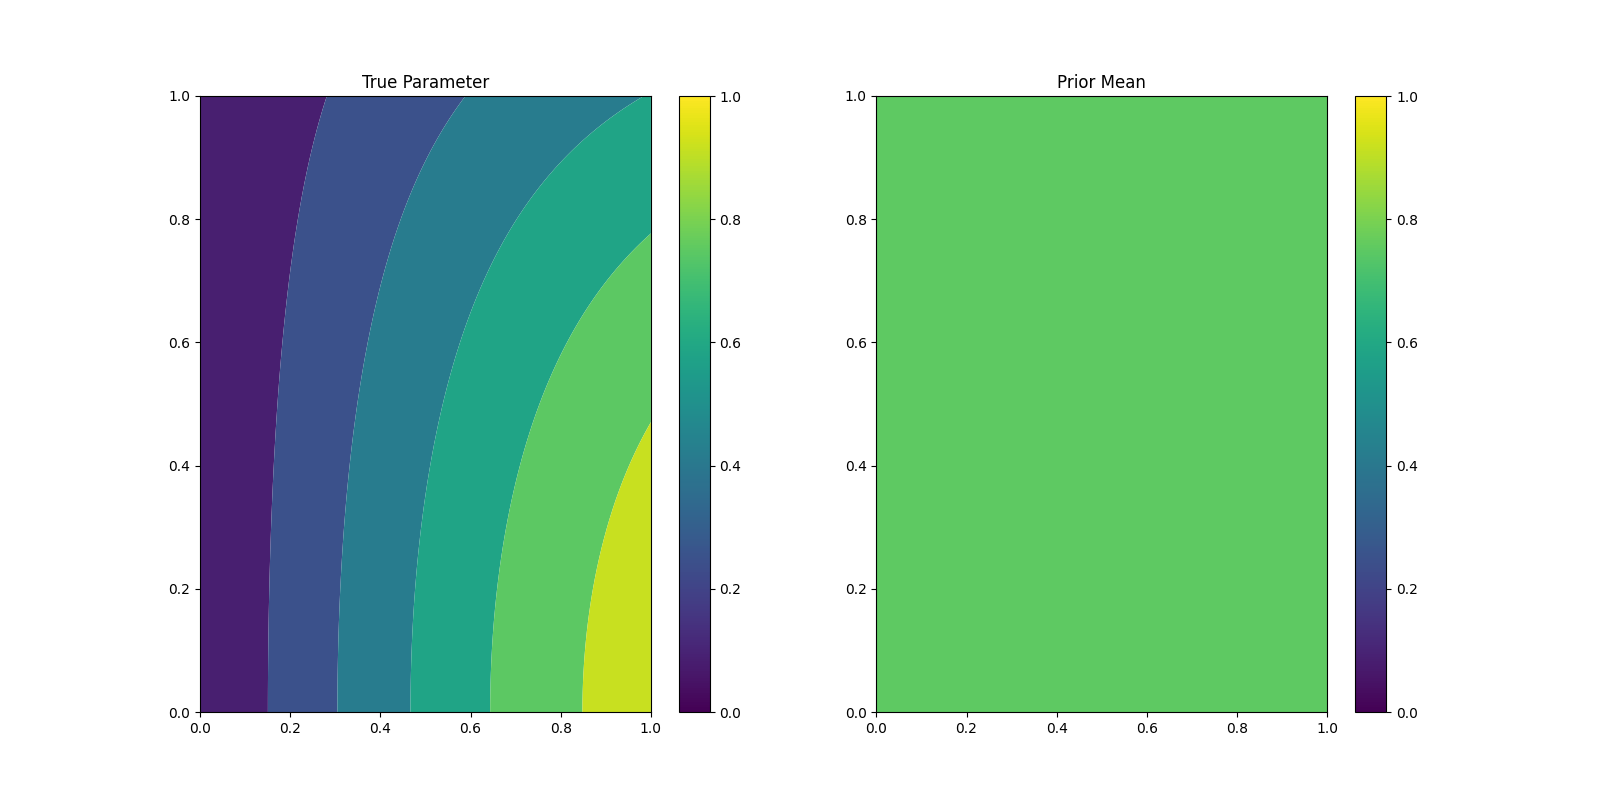
\includegraphics[width=1.0\textwidth]{figures/parameter.png}
        \caption{Variation of the true parameter and mean.}
        \label{figure:parameter}
        \end{figure}
    \item \textbf{Misfit}: \texttt{hIPPYfire} currently provides support for \texttt{ContinuousStateObservation}, which sets up the observation parameter $\mathcal{B}$. The observables which shall provide our input data are first generated by solving the forward problem by using the true parameter $\textbf{m}_{true}$
    \begin{lstlisting}[language=python]
        misfit = ContinuousStateObservation(Vh[STATE], ufl.dx, bcs=bc0)
        misfit.noise_variance = 1e-4
        utrue = pde.generate_state()
        x = [utrue, mtrue.vector(), None]
        pde.solveFwd(x[STATE], x)
        misfit.d.axpy(1., utrue)
        misfit.d.axpy(float(np.sqrt(misfit.noise_variance)), randomGen(Vh[STATE]).vector())
    \end{lstlisting}
    \begin{figure}[th]
        \centering
        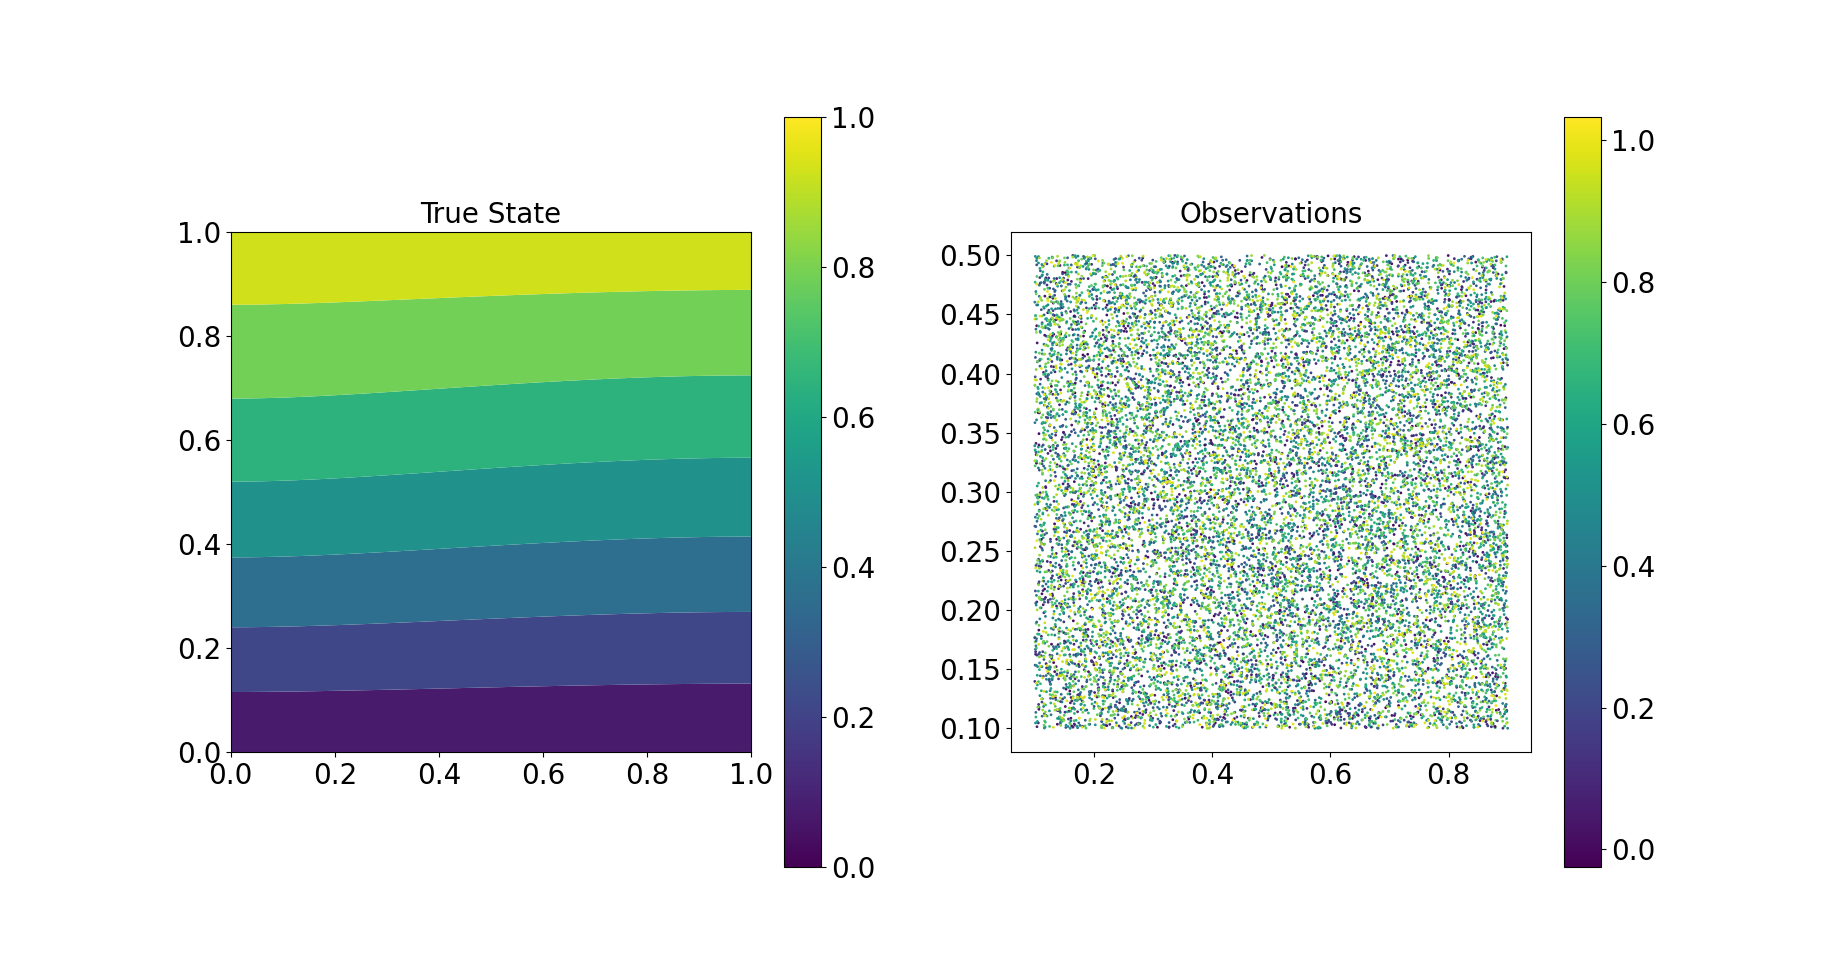
\includegraphics[width=1.0\textwidth]{figures/observations.png}
        \caption{Variation of the true state and the observations.}
        \label{figure:state}
    \end{figure}
    \item \textbf{Model}: The model, which is created by the \texttt{model} class, depends on three components---namely \texttt{PDEVariationalProblem}, \texttt{misfit}, and \texttt{prior}. The \texttt{PDEVariationalProblem} provides solutions for the forward and adjoint problems and incremental forward and adjoint problems. The \texttt{prior} applies the regularization operator to a vector, while the \texttt{misfit} computes the cost functional and partial derivatives with respect to the state and parameter variables.
    Forward finite differences are used to test the model through the \texttt{modelVerify} module.
    \begin{lstlisting}[language=python]
        model = Model(pde, pr, misfit)
        eps, err_grad, err_H = modelVerify(model, m0, misfit_only=False)
    \end{lstlisting}
    \begin{lstlisting}[language=bash]
        (yy, H xx) - (xx, H yy) =  0.0
    \end{lstlisting}
    \begin{figure}[th]
        \centering
        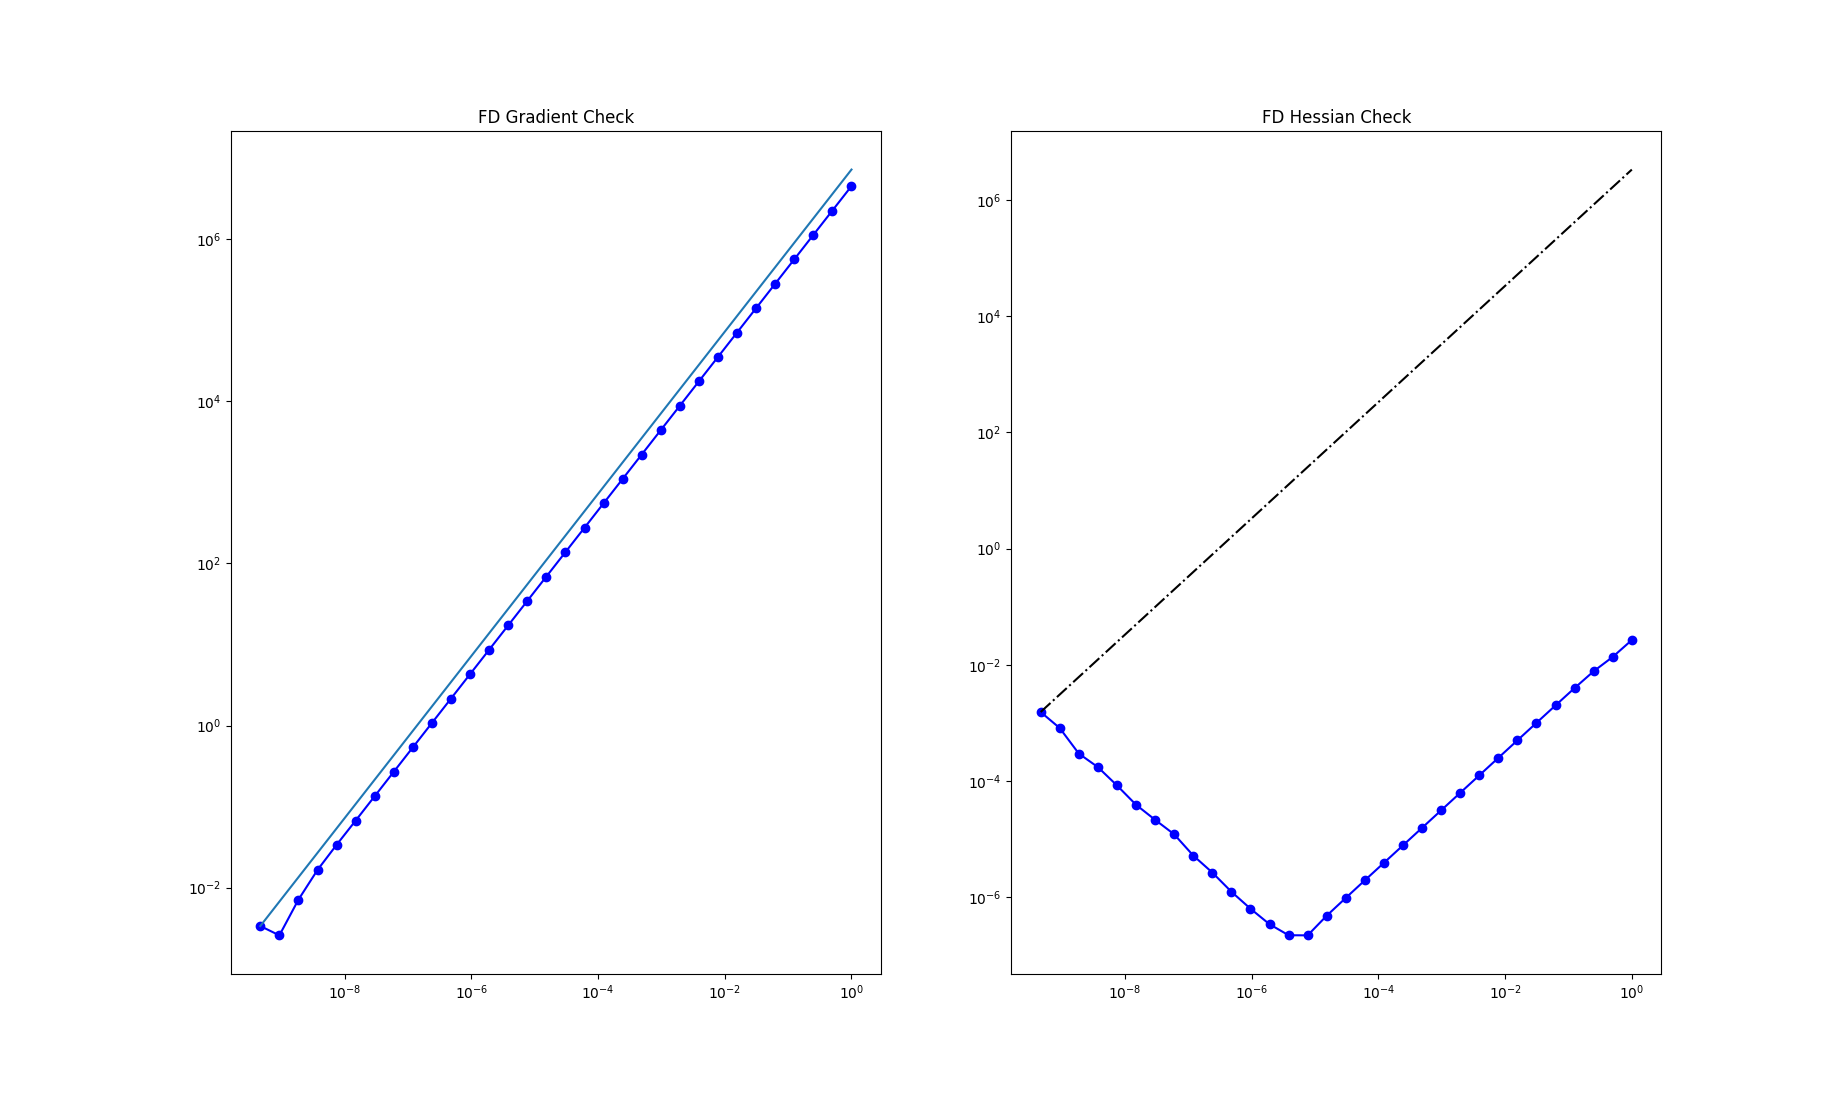
\includegraphics[width=1.0\textwidth]{figures/modelVerify.png}
        \caption{Gradient and Hessian Checks obtained from \texttt{modelVerify}}
        \label{figure:modelVerify}
    \end{figure}
    \item \textbf{MAP Point}: The Newton-CG method is used to compute the MAP point.
    \begin{lstlisting}[language=python]
        m = pr.mean.copy()
        solver = ReducedSpaceNewtonCG(model)
        solver.parameters["rel_tolerance"] = 1e-6
        solver.parameters["abs_tolerance"] = 1e-12
        solver.parameters["max_iter"]      = 25
        solver.parameters["GN_iter"] = 5
        solver.parameters["globalization"] = "LS"
        solver.parameters["LS"]["c_armijo"] = 1e-4
        x = solver.solve([None, m, None])
    \end{lstlisting}
    The following output was obtained:
    \begin{lstlisting}[language=bash]
        Relative/Absolute residual less than tol
Converged in  19  iterations with final norm  5.65259722013104e-08

It  cg_it cost            misfit          reg             (g,dm)          ||g||L2        alpha          tolcg         
1   1    9.452277e-01    8.990612e-01    4.616652e-02   -2.456844e+01   1.685316e+02   1.000000e+00   5.000000e-01
2   2    4.228824e-01    3.488744e-01    7.400803e-02   -1.043988e+00   1.715492e+01   1.000000e+00   3.190463e-01
3   5    4.027649e-01    3.196818e-01    8.308311e-02   -4.042007e-02   3.036538e+00   1.000000e+00   1.342297e-01
4   7    4.026241e-01    3.196381e-01    8.298594e-02   -3.009693e-04   2.404168e-01   1.000000e+00   3.776954e-02
5   7    4.026228e-01    3.196101e-01    8.301271e-02   -2.859017e-06   1.569884e-02   1.000000e+00   9.651461e-03
6   8    4.026228e-01    3.196134e-01    8.300935e-02   -4.118272e-08   8.007385e-04   1.000000e+00   2.179740e-03
5.941225051879883 Executiion time

Converged in  6  iterations.
Termination reason:  Norm of the gradient less than tolerance
Final gradient norm:  7.784347671669573e-06
Final cost:  0.40262278305284716
    \end{lstlisting}
    \begin{figure}[th]
        \centering
        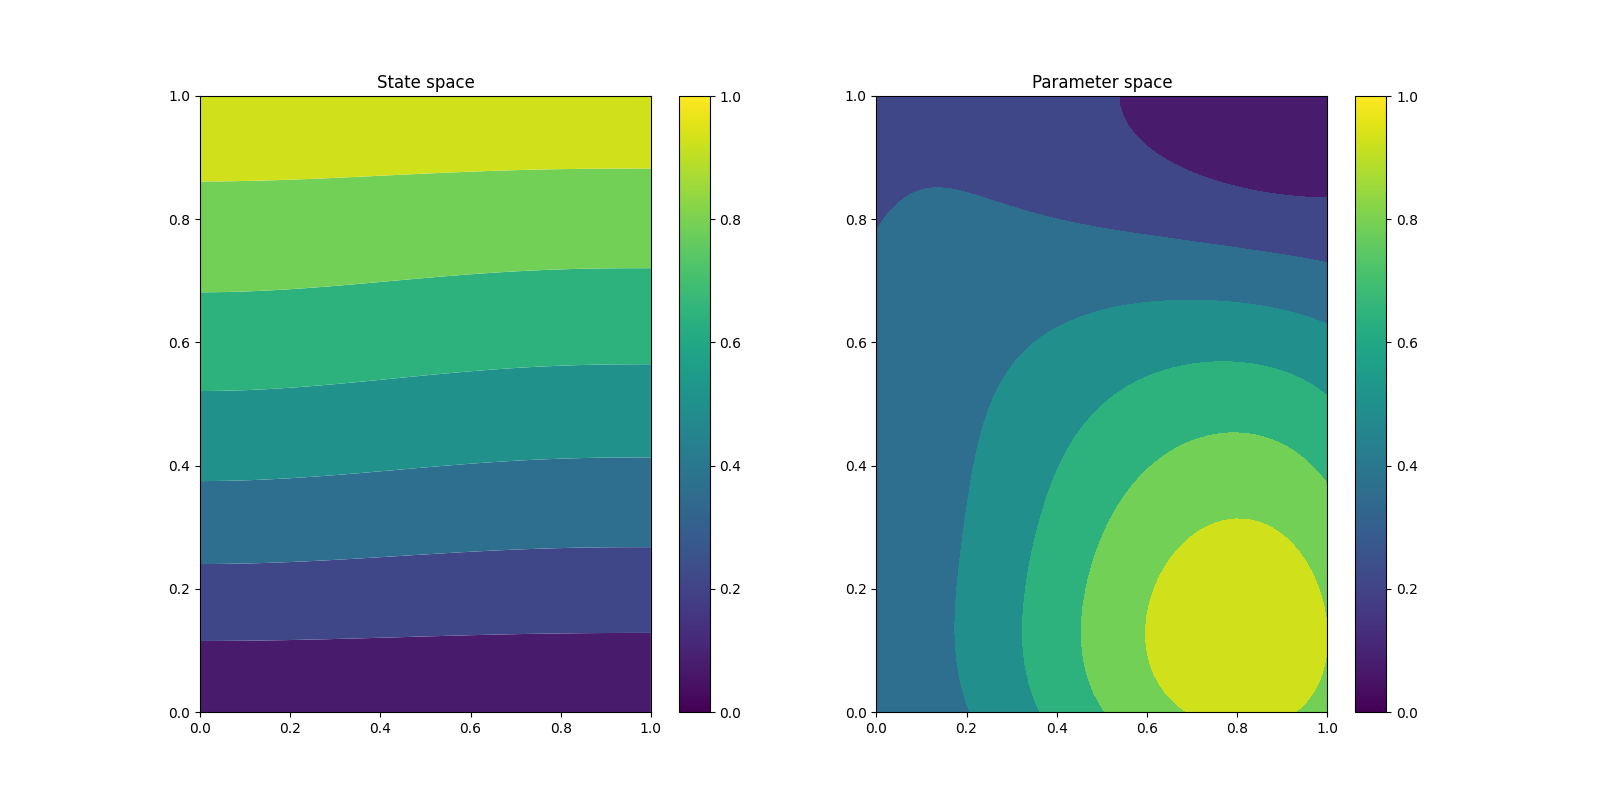
\includegraphics[width=1.0\textwidth]{figures/space.png}
        \caption{Contours of the state and parameter}
        \label{figure:space}
    \end{figure}
    A mesh independence study was conducted to establish that the convergence of the problem is observed for different sizes. The current sample assumes a uniform square mesh with 64 divisions. Experiments were conducted for mesh sizes of 128 and 256 divisions. Convergence was reported for 6--7 iterations for all mesh sizes. 
\end{itemize}
\chapter{Conclusion}
\label{chapter:conclusion}
% \chapter{Using This Template}

This chapter discusses the anatomy of \texttt{main.tex}, the file that is compiled to produce the actual report.

\section{Preamble} % ==========================================================

The \emph{preamble} of a \texttt{.tex} file is everything that comes before \verb+\begin{document}+.
\index{preamble}

\subsection{Configuration} % --------------------------------------------------

The document \texttt{main.tex} starts with the following lines.
\begin{verbatim}
    \documentclass[12pt]{report}
    \usepackage{utdiss}
    % Imports ---------------------------------------------------------------------

% Required packages.
\usepackage{amsfonts}               % Write mathematics.
\usepackage{amscd}                  % Write mathematics.
\usepackage{amsmath}                % Write mathematics.
\usepackage{amsthm}                 % Write mathematics.
\usepackage{graphicx}               % Include figures from external files.
\usepackage{lmodern}                % Handle font sizes.
\usepackage{makeidx}                % For making an index.
\usepackage{hyperref}               % Embed hyperlinks in the PDF.
\usepackage[nameinlink]{cleveref}   % Make references with \cref{}.
% NOTE: hyperref must be imported BEFORE cleveref.

% Optional packages.
% \usepackage{draftwatermark}       % "DRAFT" watermark in background.

% Packages used solely for the explanation in the template.
\usepackage{layout}                 % Draw the page layout with \layout*.
\usepackage{url}                    % Typesetting URLs.
\usepackage{verbatim}               % Quote block of text verbatim.

% Hyperlink setup -------------------------------------------------------------

\hypersetup{colorlinks=true,allcolors=black}

% Page setup ------------------------------------------------------------------

%% Line spacing (uncomment one).
% \singlespacing \singlespacequote
% \oneandonehalfspacing \oneandonehalfspacequote        % DEFAULT
% \doublespacing \doublespacequote

% Math environments -----------------------------------------------------------

\theoremstyle{plain}        % If changed, also change line 280 of utdiss.sty.
\newtheorem{theorem}{Theorem}[chapter]                  % Number by chapter
\newtheorem{corollary}[theorem]{Corollary}
\newtheorem{lemma}[theorem]{Lemma}
\newtheorem{proposition}[theorem]{Proposition}

\theoremstyle{definition}
\newtheorem{definition}[theorem]{Definition}

\theoremstyle{remark}
\newtheorem{remark}[theorem]{Remark}
\newtheorem*{notation}{Notation}

% Number equations by chapter (Theorem 2.1, 2.2, ...).
\numberwithin{equation}{chapter}
\crefformat{equation}{#2(#1)#3}

% Other customizations --------------------------------------------------------
\usepackage{amssymb,latexsym,amsfonts,amsmath,amsthm, }
\usepackage{graphicx}
\numberwithin{equation}{section}
\newtheorem{example}[theorem]{Example}
\usepackage{minted}
\usepackage[T1]{fontenc}
\usepackage{float}
\usepackage{algorithm}
\usepackage{algorithmic}

\usepackage{minted}
\usepackage{bm}
\usepackage{hyperref}
\usepackage{listings}
\usepackage{xcolor}
\usepackage{soul}

\definecolor{codegreen}{rgb}{0,0.6,0}
\definecolor{codegray}{rgb}{0.5,0.5,0.5}
\definecolor{codepurple}{rgb}{0.58,0,0.82}
\definecolor{backcolour}{rgb}{0.95,0.95,0.92}

\lstdefinestyle{mystyle}{
    backgroundcolor=\color{backcolour},   
    commentstyle=\color{codegreen},
    keywordstyle=\color{magenta},
    numberstyle=\tiny\color{codegray},
    stringstyle=\color{codepurple},
    basicstyle=\ttfamily\footnotesize,
    breakatwhitespace=false,         
    breaklines=true,                 
    captionpos=b,                    
    keepspaces=true,                 
    numbers=left,                    
    numbersep=2pt,                  
    showspaces=false,                
    showstringspaces=false,
    showtabs=false,                  
    tabsize=1
}

\lstset{style=mystyle}

\end{verbatim}

The first line, \verb+\documentclass[12pt]{report}+, declares \texttt{report} as the document class with an option of 12pt for the character size (which is slightly greater that the default 10pt, but it's what the Office of the Graduate School recommends).
You may include other options, as in any other \LaTeX{} document.

The second line, \verb+\usepackage{utdiss}+, loads the \texttt{utdiss} package, which contains a set of commands intended to produce a document fulfilling the official requirements for a doctoral dissertation or master's thesis or report.

The third line, \verb+% Imports ---------------------------------------------------------------------

% Required packages.
\usepackage{amsfonts}               % Write mathematics.
\usepackage{amscd}                  % Write mathematics.
\usepackage{amsmath}                % Write mathematics.
\usepackage{amsthm}                 % Write mathematics.
\usepackage{graphicx}               % Include figures from external files.
\usepackage{lmodern}                % Handle font sizes.
\usepackage{makeidx}                % For making an index.
\usepackage{hyperref}               % Embed hyperlinks in the PDF.
\usepackage[nameinlink]{cleveref}   % Make references with \cref{}.
% NOTE: hyperref must be imported BEFORE cleveref.

% Optional packages.
% \usepackage{draftwatermark}       % "DRAFT" watermark in background.

% Packages used solely for the explanation in the template.
\usepackage{layout}                 % Draw the page layout with \layout*.
\usepackage{url}                    % Typesetting URLs.
\usepackage{verbatim}               % Quote block of text verbatim.

% Hyperlink setup -------------------------------------------------------------

\hypersetup{colorlinks=true,allcolors=black}

% Page setup ------------------------------------------------------------------

%% Line spacing (uncomment one).
% \singlespacing \singlespacequote
% \oneandonehalfspacing \oneandonehalfspacequote        % DEFAULT
% \doublespacing \doublespacequote

% Math environments -----------------------------------------------------------

\theoremstyle{plain}        % If changed, also change line 280 of utdiss.sty.
\newtheorem{theorem}{Theorem}[chapter]                  % Number by chapter
\newtheorem{corollary}[theorem]{Corollary}
\newtheorem{lemma}[theorem]{Lemma}
\newtheorem{proposition}[theorem]{Proposition}

\theoremstyle{definition}
\newtheorem{definition}[theorem]{Definition}

\theoremstyle{remark}
\newtheorem{remark}[theorem]{Remark}
\newtheorem*{notation}{Notation}

% Number equations by chapter (Theorem 2.1, 2.2, ...).
\numberwithin{equation}{chapter}
\crefformat{equation}{#2(#1)#3}

% Other customizations --------------------------------------------------------
\usepackage{amssymb,latexsym,amsfonts,amsmath,amsthm, }
\usepackage{graphicx}
\numberwithin{equation}{section}
\newtheorem{example}[theorem]{Example}
\usepackage{minted}
\usepackage[T1]{fontenc}
\usepackage{float}
\usepackage{algorithm}
\usepackage{algorithmic}

\usepackage{minted}
\usepackage{bm}
\usepackage{hyperref}
\usepackage{listings}
\usepackage{xcolor}
\usepackage{soul}

\definecolor{codegreen}{rgb}{0,0.6,0}
\definecolor{codegray}{rgb}{0.5,0.5,0.5}
\definecolor{codepurple}{rgb}{0.58,0,0.82}
\definecolor{backcolour}{rgb}{0.95,0.95,0.92}

\lstdefinestyle{mystyle}{
    backgroundcolor=\color{backcolour},   
    commentstyle=\color{codegreen},
    keywordstyle=\color{magenta},
    numberstyle=\tiny\color{codegray},
    stringstyle=\color{codepurple},
    basicstyle=\ttfamily\footnotesize,
    breakatwhitespace=false,         
    breaklines=true,                 
    captionpos=b,                    
    keepspaces=true,                 
    numbers=left,                    
    numbersep=2pt,                  
    showspaces=false,                
    showstringspaces=false,
    showtabs=false,                  
    tabsize=1
}

\lstset{style=mystyle}
+, executes \texttt{config.tex}, which contains package imports and other customizations.
This is the file that you should put any customizations like \verb+\newcommand{}+ macros.
Note that \texttt{config.tex} is where the line spacing is set, chosen by uncommenting \textbf{one} of the following lines.
\begin{verbatim}
    % \singlespacing \singlespacequote
    % \oneandonehalfspacing \oneandonehalfspacequote
    % \doublespacing \doublespacequote
\end{verbatim}
\index{commands!singlespacing@\verb+\singlespacing+}%
\index{commands!singlespacequote@\verb+\singlespacequote+}%
\index{commands!oneandonehalfspacing@\verb+\oneandonehalfspacing+}%
\index{commands!oneandonehalfspacequote@\verb+\oneandonehalfspacequote+}%
\index{commands!doublespacing@\verb+\doublespacing+}%
\index{commands!doublespacequote@\verb+\doublespacequote+}%
At the time of writing, the Graduate School recommends at least one-and-a-half spacing.

\subsection{Author Data} % -----------------------------------------------------

The remainder of the preamble gathers data about the author and the committee.
\begin{verbatim}
    \author{First Middle Last}
    \address{youremail@utexas.edu}
    \title{Title of Your Dissertation or Thesis}

    \supervisor{Supervisor Name}
    \committeemembers
        [Committee Member B]
        [Committee Member C]
        [Committee Member D]
        {Committee Member E}        % Note the curly braces!

    \previousdegrees{B.S., M.S.}
    \graduationmonth{May}
    \graduationyear{2023}
    \typist{the author}
\end{verbatim}
Most of these commands are self explanatory.
Some details:

\begin{itemize}
    \item \verb+\author{}+: \index{commands!author@\verb+\author{}+}%
    Your full, official University name.
    Mixed case (e.g., \texttt{McCluskey}) is fine.

    \item \verb+\address{}+: \index{commands!address@\verb+\address{}+}%
    An email address \textbf{that you will still be able to use after graduation}.
    The Graduate School recommends \textbf{not} using a physical address for privacy/security reasons.

    \item \verb+\title{}+: \index{commands!title@\verb+\title{}+}%
    Your dissertation title.
    If the title consists of more than one line, it should be in inverted pyramid form.
    You may have to specify the line breakings by inserting newlines with \verb+\\+ or \verb+\newline+.

    \item \verb+\supervisor{}+: \index{commands!supervisor@\verb+\supervisor{}+}%
    The name of your advisor, i.e., the chair of your committee.
    If you have co-supervisors, use \verb+\supervisor[First Supervisor]{Second Supervisor}+.

    \item \verb+\committeemembers{}+: \index{commands!committee@\verb+\committeemembers[]{}+}%
    The names of the members of your committee, in the order that you want them to appear.
    Each name is surrounded in brackets \verb"[]" except for the final name, which goes in curly braces \verb"{}".

    \item \verb+\previousdegrees{}+: \index{commands!previousdegrees@\verb+\previousdegrees{}+}%
    Your previous degree(s), i.e., \texttt{B.S.} or \texttt{B.S., M.S.} or similar.

    \item \verb+\graduationmonth{}+: \index{commands!graduationmonth@\verb+\graduationmonth{}+}%
    The month of your graduation (May, August, or December).
    Do not abbreviate the month.

    \item \verb+\graduationyear{}+: \index{commands!graduationyear@\verb+\graduationyear{}+}%
    The year of your graduation.
    Use a 4 digit number (e.g., \texttt{2023}).

    \item \verb+\typist{}+: \index{commands!typist@\verb+\typist{}+}%
    The person who typed this report.
    If you do it yourself, put ``\texttt{the author}''.
\end{itemize}

The preamble concludes with \verb+\makeindex+.
Leave that command there, even if you do not have an index as described in \Cref{sec:usage:index}

\subsection{Modifications for Master's Degrees} % -----------------------------

Reports and theses for master's degrees must also include \verb+\degree{}+ and \verb+\degreeabbr{}+ commands and EITHER \verb+\masterthesis+ OR \verb+\masterreport+ before \verb+\makeindex+.
\begin{verbatim}
    \degree{MASTER OF SCIENCE}          % Or MASTER OF ARTS, for example.
    \degreeabbr{M.S.}                   % Or M.A., for example.
    % \masterthesis                     % Uncomment ONE of these.
    % \masterreport                     % Uncomment ONE of these.
\end{verbatim}
\index{master's degree!thesis}
\index{master's degree!report}
\index{commands!degree@\verb+\degree{}+}
\index{commands!degreeabbr@\verb+\degreeabbr{}+}
\index{commands!masterthesis@\verb+\masterthesis+}
\index{commands!masterreport@\verb+\masterreport+}
By default the document is formated as a doctoral dissertation.

In addition, the \verb+\titlepage+ command must come before the \verb+\commcertpage+ command (see next section).

\section{Front Matter} % =======================================================

Immediately after \verb+\begin{document}+ are the following lines.
\begin{verbatim}
    \copyrightpage
    \commcertpage
    \titlepage

    \begin{dedication}
    A short dedication to someone special.
    \end{dedication}

    \begin{acknowledgments}
    Acknowledgments are technically optional, but come on, it takes a village. Say thanks!
\index{Acknowledgments@\emph{Acknowledgments}}
This section is not limited to a single page.

This \LaTeX{} template was originally written in 1991 by Young~U.~Ryu and later modified by Miguel~A.~Lerma and Craig~McCluskey.
Thanks you guys, we all owe you.
The template was heavily modified by Shane~A.~McQuarrie in 2023.
\index{template!history of}

    \end{acknowledgments}

    \utabstract
    \indent
    \index{Abstract@\emph{Abstract}}
This study presents the implementation of \texttt{hIPPYfire}, a solver for large-scale Bayesian and deterministic inverse problems governed by partial differential equations (PDEs) with infinite-dimensional parameter fields that become high-dimensional after discretization. It utilizes the same scalable algorithms introduced by its predecessor, \texttt{hIPPYlib}, such as the inexact Newton Conjugate Gradient (Newton-CG) method for the computation of the maximum \textit{aposteriori} distribution (MAP point) and the low rank-approximation of the Hessian. These algorithms exploit the fact that several PDE models of physical systems have a low-dimensional solution manifold. \texttt{hIPPYfire} computes the solution of the inverse problem at a cost independent of the parameter dimension, which is measured in terms of the number of linear forward PDE solves. However, unlike \texttt{hIPPYlib} (which is built on FEniCS), \texttt{hIPPYfire} uses Firedrake to solve the PDE governing the forward problem. Firedrake presents a unique modular structure that clearly distinguishes between the programming and mathematical aspects of the library---thereby enabling contributions from programmers and mathematicians alike and ensuring its consistent development. The functionality of the solver is validated by running it on an inverse problem that is governed by an elliptic PDE according to the Bayesian framework. The major components of the inverse problem, namely the forward problem, misfit, and prior functionals, are clearly defined and used to compute the solution of the forward problem and calculate the MAP point using the inexact Newton-CG method. The succesful computation of the forward problem solution and MAP point, coupled with the efficient abstraction in Firedrake, provide motivation to incorporate functionality into \texttt{hIPPYfire}, such as the low-rank approximations of the posterior covariance and the Hessian of the data misfit.


    \tableofcontents
    \listoftables
    \listoffigures
\end{verbatim}
\index{commands!copyrightpage@\verb+\copyrightpage+}
\index{commands!commcertpage@\verb+\commcertpage+}
\index{commands!titlepage@\verb+\titlepage+}
\index{environments!dedication@\verb+dedication+}
\index{environments!acknowledgments@\verb+acknowledgments+}
\index{commands!utabstract@\verb+\utabstract+}
\index{commands!tableofcontents@\verb+\tableofcontents+}
\index{commands!listoftables@\verb+\listoftables+}
\index{commands!listoffigures@\verb+\listoffigures+}
Leave these lines alone except for the dedication, the lines between \verb+\begin{dedication}+ and \verb+\end{dedication}+.
Write something short, sweet, and possibly heartwarming within the \verb+\emph{}+.

The text of the abstract should be placed in \texttt{abstract.tex}.
Similarly, the text of the acknowledgments should be placed in \texttt{acknowledgments.tex}.

If there are 10 or more sections, 10 or more subsections for a section,
etc., you need adjust to the Table of Contents by using the
command \verb+\longtocentry+.
\index{commands!longtocentry@\verb+\longtocentry+}%
This command allocates the proper horizontal space for double-digit
numbers.

\section{Body} % ==============================================================

We've finally arrived at the actual text of the report, which should be organized into chapters and appendices.
If you are writing a short dissertation
that does not require chapters, use the command \verb+\nochapters+
\index{commands!nochapters@\verb+\nochapters+}%
Otherwise, we strongly recommend\footnote{See \url{https://www.overleaf.com/learn/latex/Management_in_a_large_project}.} placing the source text for each chapter or appendix in its own files to allow chapters to be easily inserted, re-ordered, or removed.
This way, the next chunk of \texttt{main.tex} will then looks something like this:
\begin{verbatim}
    \include{chapter-introduction}
    \chapter{Using This Template}

This chapter discusses the anatomy of \texttt{main.tex}, the file that is compiled to produce the actual report.

\section{Preamble} % ==========================================================

The \emph{preamble} of a \texttt{.tex} file is everything that comes before \verb+\begin{document}+.
\index{preamble}

\subsection{Configuration} % --------------------------------------------------

The document \texttt{main.tex} starts with the following lines.
\begin{verbatim}
    \documentclass[12pt]{report}
    \usepackage{utdiss}
    % Imports ---------------------------------------------------------------------

% Required packages.
\usepackage{amsfonts}               % Write mathematics.
\usepackage{amscd}                  % Write mathematics.
\usepackage{amsmath}                % Write mathematics.
\usepackage{amsthm}                 % Write mathematics.
\usepackage{graphicx}               % Include figures from external files.
\usepackage{lmodern}                % Handle font sizes.
\usepackage{makeidx}                % For making an index.
\usepackage{hyperref}               % Embed hyperlinks in the PDF.
\usepackage[nameinlink]{cleveref}   % Make references with \cref{}.
% NOTE: hyperref must be imported BEFORE cleveref.

% Optional packages.
% \usepackage{draftwatermark}       % "DRAFT" watermark in background.

% Packages used solely for the explanation in the template.
\usepackage{layout}                 % Draw the page layout with \layout*.
\usepackage{url}                    % Typesetting URLs.
\usepackage{verbatim}               % Quote block of text verbatim.

% Hyperlink setup -------------------------------------------------------------

\hypersetup{colorlinks=true,allcolors=black}

% Page setup ------------------------------------------------------------------

%% Line spacing (uncomment one).
% \singlespacing \singlespacequote
% \oneandonehalfspacing \oneandonehalfspacequote        % DEFAULT
% \doublespacing \doublespacequote

% Math environments -----------------------------------------------------------

\theoremstyle{plain}        % If changed, also change line 280 of utdiss.sty.
\newtheorem{theorem}{Theorem}[chapter]                  % Number by chapter
\newtheorem{corollary}[theorem]{Corollary}
\newtheorem{lemma}[theorem]{Lemma}
\newtheorem{proposition}[theorem]{Proposition}

\theoremstyle{definition}
\newtheorem{definition}[theorem]{Definition}

\theoremstyle{remark}
\newtheorem{remark}[theorem]{Remark}
\newtheorem*{notation}{Notation}

% Number equations by chapter (Theorem 2.1, 2.2, ...).
\numberwithin{equation}{chapter}
\crefformat{equation}{#2(#1)#3}

% Other customizations --------------------------------------------------------
\usepackage{amssymb,latexsym,amsfonts,amsmath,amsthm, }
\usepackage{graphicx}
\numberwithin{equation}{section}
\newtheorem{example}[theorem]{Example}
\usepackage{minted}
\usepackage[T1]{fontenc}
\usepackage{float}
\usepackage{algorithm}
\usepackage{algorithmic}

\usepackage{minted}
\usepackage{bm}
\usepackage{hyperref}
\usepackage{listings}
\usepackage{xcolor}
\usepackage{soul}

\definecolor{codegreen}{rgb}{0,0.6,0}
\definecolor{codegray}{rgb}{0.5,0.5,0.5}
\definecolor{codepurple}{rgb}{0.58,0,0.82}
\definecolor{backcolour}{rgb}{0.95,0.95,0.92}

\lstdefinestyle{mystyle}{
    backgroundcolor=\color{backcolour},   
    commentstyle=\color{codegreen},
    keywordstyle=\color{magenta},
    numberstyle=\tiny\color{codegray},
    stringstyle=\color{codepurple},
    basicstyle=\ttfamily\footnotesize,
    breakatwhitespace=false,         
    breaklines=true,                 
    captionpos=b,                    
    keepspaces=true,                 
    numbers=left,                    
    numbersep=2pt,                  
    showspaces=false,                
    showstringspaces=false,
    showtabs=false,                  
    tabsize=1
}

\lstset{style=mystyle}

\end{verbatim}

The first line, \verb+\documentclass[12pt]{report}+, declares \texttt{report} as the document class with an option of 12pt for the character size (which is slightly greater that the default 10pt, but it's what the Office of the Graduate School recommends).
You may include other options, as in any other \LaTeX{} document.

The second line, \verb+\usepackage{utdiss}+, loads the \texttt{utdiss} package, which contains a set of commands intended to produce a document fulfilling the official requirements for a doctoral dissertation or master's thesis or report.

The third line, \verb+% Imports ---------------------------------------------------------------------

% Required packages.
\usepackage{amsfonts}               % Write mathematics.
\usepackage{amscd}                  % Write mathematics.
\usepackage{amsmath}                % Write mathematics.
\usepackage{amsthm}                 % Write mathematics.
\usepackage{graphicx}               % Include figures from external files.
\usepackage{lmodern}                % Handle font sizes.
\usepackage{makeidx}                % For making an index.
\usepackage{hyperref}               % Embed hyperlinks in the PDF.
\usepackage[nameinlink]{cleveref}   % Make references with \cref{}.
% NOTE: hyperref must be imported BEFORE cleveref.

% Optional packages.
% \usepackage{draftwatermark}       % "DRAFT" watermark in background.

% Packages used solely for the explanation in the template.
\usepackage{layout}                 % Draw the page layout with \layout*.
\usepackage{url}                    % Typesetting URLs.
\usepackage{verbatim}               % Quote block of text verbatim.

% Hyperlink setup -------------------------------------------------------------

\hypersetup{colorlinks=true,allcolors=black}

% Page setup ------------------------------------------------------------------

%% Line spacing (uncomment one).
% \singlespacing \singlespacequote
% \oneandonehalfspacing \oneandonehalfspacequote        % DEFAULT
% \doublespacing \doublespacequote

% Math environments -----------------------------------------------------------

\theoremstyle{plain}        % If changed, also change line 280 of utdiss.sty.
\newtheorem{theorem}{Theorem}[chapter]                  % Number by chapter
\newtheorem{corollary}[theorem]{Corollary}
\newtheorem{lemma}[theorem]{Lemma}
\newtheorem{proposition}[theorem]{Proposition}

\theoremstyle{definition}
\newtheorem{definition}[theorem]{Definition}

\theoremstyle{remark}
\newtheorem{remark}[theorem]{Remark}
\newtheorem*{notation}{Notation}

% Number equations by chapter (Theorem 2.1, 2.2, ...).
\numberwithin{equation}{chapter}
\crefformat{equation}{#2(#1)#3}

% Other customizations --------------------------------------------------------
\usepackage{amssymb,latexsym,amsfonts,amsmath,amsthm, }
\usepackage{graphicx}
\numberwithin{equation}{section}
\newtheorem{example}[theorem]{Example}
\usepackage{minted}
\usepackage[T1]{fontenc}
\usepackage{float}
\usepackage{algorithm}
\usepackage{algorithmic}

\usepackage{minted}
\usepackage{bm}
\usepackage{hyperref}
\usepackage{listings}
\usepackage{xcolor}
\usepackage{soul}

\definecolor{codegreen}{rgb}{0,0.6,0}
\definecolor{codegray}{rgb}{0.5,0.5,0.5}
\definecolor{codepurple}{rgb}{0.58,0,0.82}
\definecolor{backcolour}{rgb}{0.95,0.95,0.92}

\lstdefinestyle{mystyle}{
    backgroundcolor=\color{backcolour},   
    commentstyle=\color{codegreen},
    keywordstyle=\color{magenta},
    numberstyle=\tiny\color{codegray},
    stringstyle=\color{codepurple},
    basicstyle=\ttfamily\footnotesize,
    breakatwhitespace=false,         
    breaklines=true,                 
    captionpos=b,                    
    keepspaces=true,                 
    numbers=left,                    
    numbersep=2pt,                  
    showspaces=false,                
    showstringspaces=false,
    showtabs=false,                  
    tabsize=1
}

\lstset{style=mystyle}
+, executes \texttt{config.tex}, which contains package imports and other customizations.
This is the file that you should put any customizations like \verb+\newcommand{}+ macros.
Note that \texttt{config.tex} is where the line spacing is set, chosen by uncommenting \textbf{one} of the following lines.
\begin{verbatim}
    % \singlespacing \singlespacequote
    % \oneandonehalfspacing \oneandonehalfspacequote
    % \doublespacing \doublespacequote
\end{verbatim}
\index{commands!singlespacing@\verb+\singlespacing+}%
\index{commands!singlespacequote@\verb+\singlespacequote+}%
\index{commands!oneandonehalfspacing@\verb+\oneandonehalfspacing+}%
\index{commands!oneandonehalfspacequote@\verb+\oneandonehalfspacequote+}%
\index{commands!doublespacing@\verb+\doublespacing+}%
\index{commands!doublespacequote@\verb+\doublespacequote+}%
At the time of writing, the Graduate School recommends at least one-and-a-half spacing.

\subsection{Author Data} % -----------------------------------------------------

The remainder of the preamble gathers data about the author and the committee.
\begin{verbatim}
    \author{First Middle Last}
    \address{youremail@utexas.edu}
    \title{Title of Your Dissertation or Thesis}

    \supervisor{Supervisor Name}
    \committeemembers
        [Committee Member B]
        [Committee Member C]
        [Committee Member D]
        {Committee Member E}        % Note the curly braces!

    \previousdegrees{B.S., M.S.}
    \graduationmonth{May}
    \graduationyear{2023}
    \typist{the author}
\end{verbatim}
Most of these commands are self explanatory.
Some details:

\begin{itemize}
    \item \verb+\author{}+: \index{commands!author@\verb+\author{}+}%
    Your full, official University name.
    Mixed case (e.g., \texttt{McCluskey}) is fine.

    \item \verb+\address{}+: \index{commands!address@\verb+\address{}+}%
    An email address \textbf{that you will still be able to use after graduation}.
    The Graduate School recommends \textbf{not} using a physical address for privacy/security reasons.

    \item \verb+\title{}+: \index{commands!title@\verb+\title{}+}%
    Your dissertation title.
    If the title consists of more than one line, it should be in inverted pyramid form.
    You may have to specify the line breakings by inserting newlines with \verb+\\+ or \verb+\newline+.

    \item \verb+\supervisor{}+: \index{commands!supervisor@\verb+\supervisor{}+}%
    The name of your advisor, i.e., the chair of your committee.
    If you have co-supervisors, use \verb+\supervisor[First Supervisor]{Second Supervisor}+.

    \item \verb+\committeemembers{}+: \index{commands!committee@\verb+\committeemembers[]{}+}%
    The names of the members of your committee, in the order that you want them to appear.
    Each name is surrounded in brackets \verb"[]" except for the final name, which goes in curly braces \verb"{}".

    \item \verb+\previousdegrees{}+: \index{commands!previousdegrees@\verb+\previousdegrees{}+}%
    Your previous degree(s), i.e., \texttt{B.S.} or \texttt{B.S., M.S.} or similar.

    \item \verb+\graduationmonth{}+: \index{commands!graduationmonth@\verb+\graduationmonth{}+}%
    The month of your graduation (May, August, or December).
    Do not abbreviate the month.

    \item \verb+\graduationyear{}+: \index{commands!graduationyear@\verb+\graduationyear{}+}%
    The year of your graduation.
    Use a 4 digit number (e.g., \texttt{2023}).

    \item \verb+\typist{}+: \index{commands!typist@\verb+\typist{}+}%
    The person who typed this report.
    If you do it yourself, put ``\texttt{the author}''.
\end{itemize}

The preamble concludes with \verb+\makeindex+.
Leave that command there, even if you do not have an index as described in \Cref{sec:usage:index}

\subsection{Modifications for Master's Degrees} % -----------------------------

Reports and theses for master's degrees must also include \verb+\degree{}+ and \verb+\degreeabbr{}+ commands and EITHER \verb+\masterthesis+ OR \verb+\masterreport+ before \verb+\makeindex+.
\begin{verbatim}
    \degree{MASTER OF SCIENCE}          % Or MASTER OF ARTS, for example.
    \degreeabbr{M.S.}                   % Or M.A., for example.
    % \masterthesis                     % Uncomment ONE of these.
    % \masterreport                     % Uncomment ONE of these.
\end{verbatim}
\index{master's degree!thesis}
\index{master's degree!report}
\index{commands!degree@\verb+\degree{}+}
\index{commands!degreeabbr@\verb+\degreeabbr{}+}
\index{commands!masterthesis@\verb+\masterthesis+}
\index{commands!masterreport@\verb+\masterreport+}
By default the document is formated as a doctoral dissertation.

In addition, the \verb+\titlepage+ command must come before the \verb+\commcertpage+ command (see next section).

\section{Front Matter} % =======================================================

Immediately after \verb+\begin{document}+ are the following lines.
\begin{verbatim}
    \copyrightpage
    \commcertpage
    \titlepage

    \begin{dedication}
    A short dedication to someone special.
    \end{dedication}

    \begin{acknowledgments}
    Acknowledgments are technically optional, but come on, it takes a village. Say thanks!
\index{Acknowledgments@\emph{Acknowledgments}}
This section is not limited to a single page.

This \LaTeX{} template was originally written in 1991 by Young~U.~Ryu and later modified by Miguel~A.~Lerma and Craig~McCluskey.
Thanks you guys, we all owe you.
The template was heavily modified by Shane~A.~McQuarrie in 2023.
\index{template!history of}

    \end{acknowledgments}

    \utabstract
    \indent
    \index{Abstract@\emph{Abstract}}
This study presents the implementation of \texttt{hIPPYfire}, a solver for large-scale Bayesian and deterministic inverse problems governed by partial differential equations (PDEs) with infinite-dimensional parameter fields that become high-dimensional after discretization. It utilizes the same scalable algorithms introduced by its predecessor, \texttt{hIPPYlib}, such as the inexact Newton Conjugate Gradient (Newton-CG) method for the computation of the maximum \textit{aposteriori} distribution (MAP point) and the low rank-approximation of the Hessian. These algorithms exploit the fact that several PDE models of physical systems have a low-dimensional solution manifold. \texttt{hIPPYfire} computes the solution of the inverse problem at a cost independent of the parameter dimension, which is measured in terms of the number of linear forward PDE solves. However, unlike \texttt{hIPPYlib} (which is built on FEniCS), \texttt{hIPPYfire} uses Firedrake to solve the PDE governing the forward problem. Firedrake presents a unique modular structure that clearly distinguishes between the programming and mathematical aspects of the library---thereby enabling contributions from programmers and mathematicians alike and ensuring its consistent development. The functionality of the solver is validated by running it on an inverse problem that is governed by an elliptic PDE according to the Bayesian framework. The major components of the inverse problem, namely the forward problem, misfit, and prior functionals, are clearly defined and used to compute the solution of the forward problem and calculate the MAP point using the inexact Newton-CG method. The succesful computation of the forward problem solution and MAP point, coupled with the efficient abstraction in Firedrake, provide motivation to incorporate functionality into \texttt{hIPPYfire}, such as the low-rank approximations of the posterior covariance and the Hessian of the data misfit.


    \tableofcontents
    \listoftables
    \listoffigures
\end{verbatim}
\index{commands!copyrightpage@\verb+\copyrightpage+}
\index{commands!commcertpage@\verb+\commcertpage+}
\index{commands!titlepage@\verb+\titlepage+}
\index{environments!dedication@\verb+dedication+}
\index{environments!acknowledgments@\verb+acknowledgments+}
\index{commands!utabstract@\verb+\utabstract+}
\index{commands!tableofcontents@\verb+\tableofcontents+}
\index{commands!listoftables@\verb+\listoftables+}
\index{commands!listoffigures@\verb+\listoffigures+}
Leave these lines alone except for the dedication, the lines between \verb+\begin{dedication}+ and \verb+\end{dedication}+.
Write something short, sweet, and possibly heartwarming within the \verb+\emph{}+.

The text of the abstract should be placed in \texttt{abstract.tex}.
Similarly, the text of the acknowledgments should be placed in \texttt{acknowledgments.tex}.

If there are 10 or more sections, 10 or more subsections for a section,
etc., you need adjust to the Table of Contents by using the
command \verb+\longtocentry+.
\index{commands!longtocentry@\verb+\longtocentry+}%
This command allocates the proper horizontal space for double-digit
numbers.

\section{Body} % ==============================================================

We've finally arrived at the actual text of the report, which should be organized into chapters and appendices.
If you are writing a short dissertation
that does not require chapters, use the command \verb+\nochapters+
\index{commands!nochapters@\verb+\nochapters+}%
Otherwise, we strongly recommend\footnote{See \url{https://www.overleaf.com/learn/latex/Management_in_a_large_project}.} placing the source text for each chapter or appendix in its own files to allow chapters to be easily inserted, re-ordered, or removed.
This way, the next chunk of \texttt{main.tex} will then looks something like this:
\begin{verbatim}
    \include{chapter-introduction}
    \chapter{Using This Template}

This chapter discusses the anatomy of \texttt{main.tex}, the file that is compiled to produce the actual report.

\section{Preamble} % ==========================================================

The \emph{preamble} of a \texttt{.tex} file is everything that comes before \verb+\begin{document}+.
\index{preamble}

\subsection{Configuration} % --------------------------------------------------

The document \texttt{main.tex} starts with the following lines.
\begin{verbatim}
    \documentclass[12pt]{report}
    \usepackage{utdiss}
    \input{config}
\end{verbatim}

The first line, \verb+\documentclass[12pt]{report}+, declares \texttt{report} as the document class with an option of 12pt for the character size (which is slightly greater that the default 10pt, but it's what the Office of the Graduate School recommends).
You may include other options, as in any other \LaTeX{} document.

The second line, \verb+\usepackage{utdiss}+, loads the \texttt{utdiss} package, which contains a set of commands intended to produce a document fulfilling the official requirements for a doctoral dissertation or master's thesis or report.

The third line, \verb+\input{config}+, executes \texttt{config.tex}, which contains package imports and other customizations.
This is the file that you should put any customizations like \verb+\newcommand{}+ macros.
Note that \texttt{config.tex} is where the line spacing is set, chosen by uncommenting \textbf{one} of the following lines.
\begin{verbatim}
    % \singlespacing \singlespacequote
    % \oneandonehalfspacing \oneandonehalfspacequote
    % \doublespacing \doublespacequote
\end{verbatim}
\index{commands!singlespacing@\verb+\singlespacing+}%
\index{commands!singlespacequote@\verb+\singlespacequote+}%
\index{commands!oneandonehalfspacing@\verb+\oneandonehalfspacing+}%
\index{commands!oneandonehalfspacequote@\verb+\oneandonehalfspacequote+}%
\index{commands!doublespacing@\verb+\doublespacing+}%
\index{commands!doublespacequote@\verb+\doublespacequote+}%
At the time of writing, the Graduate School recommends at least one-and-a-half spacing.

\subsection{Author Data} % -----------------------------------------------------

The remainder of the preamble gathers data about the author and the committee.
\begin{verbatim}
    \author{First Middle Last}
    \address{youremail@utexas.edu}
    \title{Title of Your Dissertation or Thesis}

    \supervisor{Supervisor Name}
    \committeemembers
        [Committee Member B]
        [Committee Member C]
        [Committee Member D]
        {Committee Member E}        % Note the curly braces!

    \previousdegrees{B.S., M.S.}
    \graduationmonth{May}
    \graduationyear{2023}
    \typist{the author}
\end{verbatim}
Most of these commands are self explanatory.
Some details:

\begin{itemize}
    \item \verb+\author{}+: \index{commands!author@\verb+\author{}+}%
    Your full, official University name.
    Mixed case (e.g., \texttt{McCluskey}) is fine.

    \item \verb+\address{}+: \index{commands!address@\verb+\address{}+}%
    An email address \textbf{that you will still be able to use after graduation}.
    The Graduate School recommends \textbf{not} using a physical address for privacy/security reasons.

    \item \verb+\title{}+: \index{commands!title@\verb+\title{}+}%
    Your dissertation title.
    If the title consists of more than one line, it should be in inverted pyramid form.
    You may have to specify the line breakings by inserting newlines with \verb+\\+ or \verb+\newline+.

    \item \verb+\supervisor{}+: \index{commands!supervisor@\verb+\supervisor{}+}%
    The name of your advisor, i.e., the chair of your committee.
    If you have co-supervisors, use \verb+\supervisor[First Supervisor]{Second Supervisor}+.

    \item \verb+\committeemembers{}+: \index{commands!committee@\verb+\committeemembers[]{}+}%
    The names of the members of your committee, in the order that you want them to appear.
    Each name is surrounded in brackets \verb"[]" except for the final name, which goes in curly braces \verb"{}".

    \item \verb+\previousdegrees{}+: \index{commands!previousdegrees@\verb+\previousdegrees{}+}%
    Your previous degree(s), i.e., \texttt{B.S.} or \texttt{B.S., M.S.} or similar.

    \item \verb+\graduationmonth{}+: \index{commands!graduationmonth@\verb+\graduationmonth{}+}%
    The month of your graduation (May, August, or December).
    Do not abbreviate the month.

    \item \verb+\graduationyear{}+: \index{commands!graduationyear@\verb+\graduationyear{}+}%
    The year of your graduation.
    Use a 4 digit number (e.g., \texttt{2023}).

    \item \verb+\typist{}+: \index{commands!typist@\verb+\typist{}+}%
    The person who typed this report.
    If you do it yourself, put ``\texttt{the author}''.
\end{itemize}

The preamble concludes with \verb+\makeindex+.
Leave that command there, even if you do not have an index as described in \Cref{sec:usage:index}

\subsection{Modifications for Master's Degrees} % -----------------------------

Reports and theses for master's degrees must also include \verb+\degree{}+ and \verb+\degreeabbr{}+ commands and EITHER \verb+\masterthesis+ OR \verb+\masterreport+ before \verb+\makeindex+.
\begin{verbatim}
    \degree{MASTER OF SCIENCE}          % Or MASTER OF ARTS, for example.
    \degreeabbr{M.S.}                   % Or M.A., for example.
    % \masterthesis                     % Uncomment ONE of these.
    % \masterreport                     % Uncomment ONE of these.
\end{verbatim}
\index{master's degree!thesis}
\index{master's degree!report}
\index{commands!degree@\verb+\degree{}+}
\index{commands!degreeabbr@\verb+\degreeabbr{}+}
\index{commands!masterthesis@\verb+\masterthesis+}
\index{commands!masterreport@\verb+\masterreport+}
By default the document is formated as a doctoral dissertation.

In addition, the \verb+\titlepage+ command must come before the \verb+\commcertpage+ command (see next section).

\section{Front Matter} % =======================================================

Immediately after \verb+\begin{document}+ are the following lines.
\begin{verbatim}
    \copyrightpage
    \commcertpage
    \titlepage

    \begin{dedication}
    A short dedication to someone special.
    \end{dedication}

    \begin{acknowledgments}
    \input{acknowledgments}
    \end{acknowledgments}

    \utabstract
    \indent
    \input{abstract}

    \tableofcontents
    \listoftables
    \listoffigures
\end{verbatim}
\index{commands!copyrightpage@\verb+\copyrightpage+}
\index{commands!commcertpage@\verb+\commcertpage+}
\index{commands!titlepage@\verb+\titlepage+}
\index{environments!dedication@\verb+dedication+}
\index{environments!acknowledgments@\verb+acknowledgments+}
\index{commands!utabstract@\verb+\utabstract+}
\index{commands!tableofcontents@\verb+\tableofcontents+}
\index{commands!listoftables@\verb+\listoftables+}
\index{commands!listoffigures@\verb+\listoffigures+}
Leave these lines alone except for the dedication, the lines between \verb+\begin{dedication}+ and \verb+\end{dedication}+.
Write something short, sweet, and possibly heartwarming within the \verb+\emph{}+.

The text of the abstract should be placed in \texttt{abstract.tex}.
Similarly, the text of the acknowledgments should be placed in \texttt{acknowledgments.tex}.

If there are 10 or more sections, 10 or more subsections for a section,
etc., you need adjust to the Table of Contents by using the
command \verb+\longtocentry+.
\index{commands!longtocentry@\verb+\longtocentry+}%
This command allocates the proper horizontal space for double-digit
numbers.

\section{Body} % ==============================================================

We've finally arrived at the actual text of the report, which should be organized into chapters and appendices.
If you are writing a short dissertation
that does not require chapters, use the command \verb+\nochapters+
\index{commands!nochapters@\verb+\nochapters+}%
Otherwise, we strongly recommend\footnote{See \url{https://www.overleaf.com/learn/latex/Management_in_a_large_project}.} placing the source text for each chapter or appendix in its own files to allow chapters to be easily inserted, re-ordered, or removed.
This way, the next chunk of \texttt{main.tex} will then looks something like this:
\begin{verbatim}
    \include{chapter-introduction}
    \include{chapter-usage}
    \include{chapter-examples}
    \include{chapter-conclusion}
\end{verbatim}
\index{commands!include@\verb+\include{}+}%

\subsection{Chapters} % -------------------------------------------------------

The beginning of each chapter file should begin with a \verb+\chapter[]{}+
\index{commands!chapter@\verb+\chapter{}+}%
command, which is similar to \verb"section{}".
The part in \verb"[]" will be listed in the table of contents; the part in \verb"{}" will be printed in the body of the document.
Use \verb+\chapter{}+ (without \verb"[]") to use the same title for both the table of contents and the body.

If your chapter heading consists of more than one line, it will be automatically broken into separate lines.
If you don't like the way LaTeX breaks the chapter heading into lines, use \verb+\newheadline+ to break lines.
\textbf{Never use} \verb+\\+ \textbf{in sectional headings} (\verb+\chapter{}+, \verb+\section{}+, \verb+\subsection{}+, etc.)!
\index{commands!chapter@\verb+\chapter{}+}%
\index{commands!section@\verb+\section{}+}%
\index{commands!subsection@\verb+\subsection{}+}%

\subsection{Appendices} % -----------------------------------------------------
\index{Appendices@\emph{Appendices}}%

If you have no appendices, then proceed to the end matter.

If you have a single appendix, use \verb+\appendix+ and \textbf{do not use}
\verb+\chapter{}+ at the start of the appendix text.
\index{commands!appendix@\verb+\appendix+}
Otherwise the template will insert an extra page with only the word
`Appendix' on it and cause the actual appendix to be labeled `Appendix 1'.

If you have more than one appendix, use \verb+\appendices+
\index{commands!appendices@\verb+\appendices+}
and \verb+\include{}+ to include your appendices the same way as chapters.
Each appendix should start with \verb+\chapter{}+, which will label them `Appendix A', `Appendix B', \ldots.

\section{End Matter} % ========================================================

After the body text and appendices come the bibliography, index (optional), and vita, in that order.

\subsection{Bibliography} % ---------------------------------------------------
\label{section:bibliography}

We recommend using BiB\TeX{} to track your references.
\index{BiBTeX@BiB\TeX{}}%
Enter reference information in \texttt{references.bib} and use the \verb+\cite{}+ command to refer to them within the body.
\index{commands!cite@\verb+\cite{}+}
The following commands then create the bibliography.
\begin{verbatim}
    \bibliographystyle{plain}
    \bibliography{references}
\end{verbatim}
\index{commands!bibliography@\verb+\bibliography{}+}
If you have no references\footnote{If there are no references, is it even a dissertation?} and hence \verb+\cite{}+ is never used, comment these commands out to exclude the bibiliography.
On the other end of the spectrum, you can use the command \verb+\nocite{*}+ to print all entries in \texttt{references.bib} in the bibliography, whether or not they were actually cited.

\subsection{Index} % ----------------------------------------------------------
\label{sec:usage:index}

An index is \emph{optional}.
This template uses three ingredients to make an index:
\begin{enumerate}
    \item \verb+\usepackage{makeidx}+ in \texttt{config.tex}.
    \item \verb+\printindex+ in \texttt{main.tex}.
    \item \verb+\index{}+ commands throughout the text.
\end{enumerate}
The \verb+\index{}+ command can be used a few ways.
\index{commands!index@\verb+\index{}+}
\begin{itemize}
    \item \verb+\index{name}+ creates an entry in the index called `name'.
    \item \verb+\index{name@\texttt{label}}+ creates an entry in the index calle `\texttt{label}', placed where `name' should appear.
    \item \verb+\index{list!name}+ creates an entry called `list' and a subentry beneath it called `name'.
\end{itemize}
If you don't have an index, or if you start placing \verb+\index{}+ commands and run out of steam, simply comment out \verb+\printindex+ to remove the index (don't spend the time deleting old \verb+\index{}+ commands, ain't nobody got time for that).
\index{commands!printindex@\verb+\printindex+}

\subsection{Vita} % -----------------------------------------------------------

The vita is a brief biographical sketch of the author and should be written in \texttt{vita.tex}.
Note that the \verb"vita" environment (defined in \texttt{utdiss.sty}) uses the info in \verb+\address{}+ and \verb+\typist{}+ from the preamble to automatically generate a few final lines.
\index{commands!address@\verb+\address{}+}
\index{commands!typist@\verb+\typist{}+}

    \chapter{Examples of Content}
\label{chapter:examples}

This chapter shows some simple examples for including technical information in the body of the report via mathematics, tables, figures, and references.
If you are unfamiliar with \LaTeX{}, see \url{https://www.overleaf.com/learn/latex/Tutorials} for an excellent suite of tutorials.

\section{Writing Mathematics} % ===============================================

Here we show some examples of writing mathematics in the report and using theorem environments.

Here are some equations using the \texttt{align} environment.
\begin{align}
    \label{eq:quadratic}
    0
    &= ax^{2} + bx + c
    \\
    \label{eq:quadraticroots}
    x
    &= \frac{-b + \sqrt{b^{2} - 4ac}}{2a}
\end{align}
\index{environments!align@\verb+align+}
You can refer to equations, like \cref{eq:quadratic}, with \verb+\cref{}+.

The configuration file \texttt{config.tex} defines the following ``theorem'' environments.
\begin{itemize}
    \item \texttt{theorem}
    \index{environments!theorem@\verb+theorem+}
    \item \texttt{corollary}
    \index{environments!corollary@\verb+corollary+}
    \item \texttt{lemma}
    \index{environments!lemma@\verb+lemma+}
    \item \texttt{proposition}
    \index{environments!proposition@\verb+proposition+}
    \item \texttt{definition}
    \index{environments!definition@\verb+definition+}
    \item \texttt{remark}
    \index{environments!remark@\verb+remark+}
    \item \texttt{notation}
    \index{environments!notation@\verb+notation+}
\end{itemize}
The \texttt{proof} environment is also available by default.
\index{environments!proof@\verb+proof+}

\begin{lemma}[An Example Lemma]
\label{lemma:example}

Let $A$ and $B$ be sets with $A \subset B$.
Then $A\cap B = A$.

\begin{proof}
We must show that $A\cap B \subset A$ and $A \subset A \cap B$.
For the first, let $x \in A \cap B$.
By definition, $x \in A$, hence $A \cap B \subset A$.
For the other direction, let $y \in A$. Since $A \subset B$, $y \in B$ as well.
Thus, $y \in A \cap B$, which implies $A\cap B \subset A$.
\end{proof}
\end{lemma}

\begin{theorem}
\label{thm:example}
Theorems look just like lemmata, except they are called `Theorem' instead of `Lemma'.
\end{theorem}

\section{Making Tables} % =====================================================

The \verb"table" environment creates a table, which usually contains a \verb"tabular" environment that houses the actual table text.
The \verb"table" environment takes an optional argument to indicate the position for the table as described in \Cref{table:positions}.
\index{environments!table@\verb+table+}%
\index{environments!tabular@\verb+tabular+}%


\begin{table}[ht]
\centering
\begin{tabular}{r|l}
    argument & position
    \\ \hline
    \texttt{h} & ``here'' if possible \\
    \texttt{t} & top of the page \\
    \texttt{b} & bottom of the page \\
    \texttt{p} & on the page of floats \\
    \texttt{H} & ``here'' no matter what (requires \verb"\usepackage{float}")
\end{tabular}
\caption[Arguments for the \texttt{table} environment.]{
    Arguments for the \texttt{table} environment. It is possible to combine several of these arguments, such as \texttt{ht} (``here'' if possible, otherwise on top of the page). The default is \texttt{tbp}.
}
\label{table:positions}
\end{table}

Use \verb"\caption[short caption]{long caption}" to add a caption to the table.
\index{caption@\verb+\caption{}+}
The \texttt{short caption} is used in the List of Tables
\index{List of Tables@\emph{List of Tables}}%
while the \texttt{long caption} appears in the actual text.
Note that \verb"\label{}" must come after \verb"\caption{}" to create a label that can be referred to elsewhere in the text with \verb"\Cref{}".

\section{Including Figures} % =================================================

The \verb"figure" environment
\index{environments!figure@\verb+figure+}
creates a figure, which usually contains an \verb"\includegraphics{}" command to import the figure from an external file.
The \verb"figure" environment takes the same optional arguments as the \verb"table" environment shown in \Cref{table:positions}.

\begin{figure}[th]
    \centering
    
\includegraphics[width=.7\textwidth]{figures/oden.pdf}
    \caption[An example figure.]{This is an example of a figure.}
    \label{figure:example}
\end{figure}

Use \verb"\caption[short caption]{long caption}" to add a caption to the figure.
\index{caption@\verb+\caption{}+}
The \texttt{short caption} is used in the List of Figures
\index{List of Figures@\emph{List of Figures}}%
while the \texttt{long caption} appears in the actual text.
Note that \verb"\label{}" must come after \verb"\caption{}" to create a label that can be referred to elsewhere in the text with \verb"\Cref{}".

We recommend placing figure files in a separate \verb"figures/" folder to keep your working directory organized.


\section{Citations} % =========================================================

The bibliography is discussed in \Cref{section:bibliography}.
Use the \verb"\cite{}" command to refer to entries defined in \texttt{references.bib}:
\begin{itemize}
    \item Cite a single reference \cite{knuth1984texbook}.
    \item Cite multiple references \cite{lamport1994latex, goosens1994latex}.
\end{itemize}

    \include{chapter-conclusion}
\end{verbatim}
\index{commands!include@\verb+\include{}+}%

\subsection{Chapters} % -------------------------------------------------------

The beginning of each chapter file should begin with a \verb+\chapter[]{}+
\index{commands!chapter@\verb+\chapter{}+}%
command, which is similar to \verb"section{}".
The part in \verb"[]" will be listed in the table of contents; the part in \verb"{}" will be printed in the body of the document.
Use \verb+\chapter{}+ (without \verb"[]") to use the same title for both the table of contents and the body.

If your chapter heading consists of more than one line, it will be automatically broken into separate lines.
If you don't like the way LaTeX breaks the chapter heading into lines, use \verb+\newheadline+ to break lines.
\textbf{Never use} \verb+\\+ \textbf{in sectional headings} (\verb+\chapter{}+, \verb+\section{}+, \verb+\subsection{}+, etc.)!
\index{commands!chapter@\verb+\chapter{}+}%
\index{commands!section@\verb+\section{}+}%
\index{commands!subsection@\verb+\subsection{}+}%

\subsection{Appendices} % -----------------------------------------------------
\index{Appendices@\emph{Appendices}}%

If you have no appendices, then proceed to the end matter.

If you have a single appendix, use \verb+\appendix+ and \textbf{do not use}
\verb+\chapter{}+ at the start of the appendix text.
\index{commands!appendix@\verb+\appendix+}
Otherwise the template will insert an extra page with only the word
`Appendix' on it and cause the actual appendix to be labeled `Appendix 1'.

If you have more than one appendix, use \verb+\appendices+
\index{commands!appendices@\verb+\appendices+}
and \verb+\include{}+ to include your appendices the same way as chapters.
Each appendix should start with \verb+\chapter{}+, which will label them `Appendix A', `Appendix B', \ldots.

\section{End Matter} % ========================================================

After the body text and appendices come the bibliography, index (optional), and vita, in that order.

\subsection{Bibliography} % ---------------------------------------------------
\label{section:bibliography}

We recommend using BiB\TeX{} to track your references.
\index{BiBTeX@BiB\TeX{}}%
Enter reference information in \texttt{references.bib} and use the \verb+\cite{}+ command to refer to them within the body.
\index{commands!cite@\verb+\cite{}+}
The following commands then create the bibliography.
\begin{verbatim}
    \bibliographystyle{plain}
    \bibliography{references}
\end{verbatim}
\index{commands!bibliography@\verb+\bibliography{}+}
If you have no references\footnote{If there are no references, is it even a dissertation?} and hence \verb+\cite{}+ is never used, comment these commands out to exclude the bibiliography.
On the other end of the spectrum, you can use the command \verb+\nocite{*}+ to print all entries in \texttt{references.bib} in the bibliography, whether or not they were actually cited.

\subsection{Index} % ----------------------------------------------------------
\label{sec:usage:index}

An index is \emph{optional}.
This template uses three ingredients to make an index:
\begin{enumerate}
    \item \verb+\usepackage{makeidx}+ in \texttt{config.tex}.
    \item \verb+\printindex+ in \texttt{main.tex}.
    \item \verb+\index{}+ commands throughout the text.
\end{enumerate}
The \verb+\index{}+ command can be used a few ways.
\index{commands!index@\verb+\index{}+}
\begin{itemize}
    \item \verb+\index{name}+ creates an entry in the index called `name'.
    \item \verb+\index{name@\texttt{label}}+ creates an entry in the index calle `\texttt{label}', placed where `name' should appear.
    \item \verb+\index{list!name}+ creates an entry called `list' and a subentry beneath it called `name'.
\end{itemize}
If you don't have an index, or if you start placing \verb+\index{}+ commands and run out of steam, simply comment out \verb+\printindex+ to remove the index (don't spend the time deleting old \verb+\index{}+ commands, ain't nobody got time for that).
\index{commands!printindex@\verb+\printindex+}

\subsection{Vita} % -----------------------------------------------------------

The vita is a brief biographical sketch of the author and should be written in \texttt{vita.tex}.
Note that the \verb"vita" environment (defined in \texttt{utdiss.sty}) uses the info in \verb+\address{}+ and \verb+\typist{}+ from the preamble to automatically generate a few final lines.
\index{commands!address@\verb+\address{}+}
\index{commands!typist@\verb+\typist{}+}

    \chapter{Examples of Content}
\label{chapter:examples}

This chapter shows some simple examples for including technical information in the body of the report via mathematics, tables, figures, and references.
If you are unfamiliar with \LaTeX{}, see \url{https://www.overleaf.com/learn/latex/Tutorials} for an excellent suite of tutorials.

\section{Writing Mathematics} % ===============================================

Here we show some examples of writing mathematics in the report and using theorem environments.

Here are some equations using the \texttt{align} environment.
\begin{align}
    \label{eq:quadratic}
    0
    &= ax^{2} + bx + c
    \\
    \label{eq:quadraticroots}
    x
    &= \frac{-b + \sqrt{b^{2} - 4ac}}{2a}
\end{align}
\index{environments!align@\verb+align+}
You can refer to equations, like \cref{eq:quadratic}, with \verb+\cref{}+.

The configuration file \texttt{config.tex} defines the following ``theorem'' environments.
\begin{itemize}
    \item \texttt{theorem}
    \index{environments!theorem@\verb+theorem+}
    \item \texttt{corollary}
    \index{environments!corollary@\verb+corollary+}
    \item \texttt{lemma}
    \index{environments!lemma@\verb+lemma+}
    \item \texttt{proposition}
    \index{environments!proposition@\verb+proposition+}
    \item \texttt{definition}
    \index{environments!definition@\verb+definition+}
    \item \texttt{remark}
    \index{environments!remark@\verb+remark+}
    \item \texttt{notation}
    \index{environments!notation@\verb+notation+}
\end{itemize}
The \texttt{proof} environment is also available by default.
\index{environments!proof@\verb+proof+}

\begin{lemma}[An Example Lemma]
\label{lemma:example}

Let $A$ and $B$ be sets with $A \subset B$.
Then $A\cap B = A$.

\begin{proof}
We must show that $A\cap B \subset A$ and $A \subset A \cap B$.
For the first, let $x \in A \cap B$.
By definition, $x \in A$, hence $A \cap B \subset A$.
For the other direction, let $y \in A$. Since $A \subset B$, $y \in B$ as well.
Thus, $y \in A \cap B$, which implies $A\cap B \subset A$.
\end{proof}
\end{lemma}

\begin{theorem}
\label{thm:example}
Theorems look just like lemmata, except they are called `Theorem' instead of `Lemma'.
\end{theorem}

\section{Making Tables} % =====================================================

The \verb"table" environment creates a table, which usually contains a \verb"tabular" environment that houses the actual table text.
The \verb"table" environment takes an optional argument to indicate the position for the table as described in \Cref{table:positions}.
\index{environments!table@\verb+table+}%
\index{environments!tabular@\verb+tabular+}%


\begin{table}[ht]
\centering
\begin{tabular}{r|l}
    argument & position
    \\ \hline
    \texttt{h} & ``here'' if possible \\
    \texttt{t} & top of the page \\
    \texttt{b} & bottom of the page \\
    \texttt{p} & on the page of floats \\
    \texttt{H} & ``here'' no matter what (requires \verb"\usepackage{float}")
\end{tabular}
\caption[Arguments for the \texttt{table} environment.]{
    Arguments for the \texttt{table} environment. It is possible to combine several of these arguments, such as \texttt{ht} (``here'' if possible, otherwise on top of the page). The default is \texttt{tbp}.
}
\label{table:positions}
\end{table}

Use \verb"\caption[short caption]{long caption}" to add a caption to the table.
\index{caption@\verb+\caption{}+}
The \texttt{short caption} is used in the List of Tables
\index{List of Tables@\emph{List of Tables}}%
while the \texttt{long caption} appears in the actual text.
Note that \verb"\label{}" must come after \verb"\caption{}" to create a label that can be referred to elsewhere in the text with \verb"\Cref{}".

\section{Including Figures} % =================================================

The \verb"figure" environment
\index{environments!figure@\verb+figure+}
creates a figure, which usually contains an \verb"\includegraphics{}" command to import the figure from an external file.
The \verb"figure" environment takes the same optional arguments as the \verb"table" environment shown in \Cref{table:positions}.

\begin{figure}[th]
    \centering
    
\includegraphics[width=.7\textwidth]{figures/oden.pdf}
    \caption[An example figure.]{This is an example of a figure.}
    \label{figure:example}
\end{figure}

Use \verb"\caption[short caption]{long caption}" to add a caption to the figure.
\index{caption@\verb+\caption{}+}
The \texttt{short caption} is used in the List of Figures
\index{List of Figures@\emph{List of Figures}}%
while the \texttt{long caption} appears in the actual text.
Note that \verb"\label{}" must come after \verb"\caption{}" to create a label that can be referred to elsewhere in the text with \verb"\Cref{}".

We recommend placing figure files in a separate \verb"figures/" folder to keep your working directory organized.


\section{Citations} % =========================================================

The bibliography is discussed in \Cref{section:bibliography}.
Use the \verb"\cite{}" command to refer to entries defined in \texttt{references.bib}:
\begin{itemize}
    \item Cite a single reference \cite{knuth1984texbook}.
    \item Cite multiple references \cite{lamport1994latex, goosens1994latex}.
\end{itemize}

    \include{chapter-conclusion}
\end{verbatim}
\index{commands!include@\verb+\include{}+}%

\subsection{Chapters} % -------------------------------------------------------

The beginning of each chapter file should begin with a \verb+\chapter[]{}+
\index{commands!chapter@\verb+\chapter{}+}%
command, which is similar to \verb"section{}".
The part in \verb"[]" will be listed in the table of contents; the part in \verb"{}" will be printed in the body of the document.
Use \verb+\chapter{}+ (without \verb"[]") to use the same title for both the table of contents and the body.

If your chapter heading consists of more than one line, it will be automatically broken into separate lines.
If you don't like the way LaTeX breaks the chapter heading into lines, use \verb+\newheadline+ to break lines.
\textbf{Never use} \verb+\\+ \textbf{in sectional headings} (\verb+\chapter{}+, \verb+\section{}+, \verb+\subsection{}+, etc.)!
\index{commands!chapter@\verb+\chapter{}+}%
\index{commands!section@\verb+\section{}+}%
\index{commands!subsection@\verb+\subsection{}+}%

\subsection{Appendices} % -----------------------------------------------------
\index{Appendices@\emph{Appendices}}%

If you have no appendices, then proceed to the end matter.

If you have a single appendix, use \verb+\appendix+ and \textbf{do not use}
\verb+\chapter{}+ at the start of the appendix text.
\index{commands!appendix@\verb+\appendix+}
Otherwise the template will insert an extra page with only the word
`Appendix' on it and cause the actual appendix to be labeled `Appendix 1'.

If you have more than one appendix, use \verb+\appendices+
\index{commands!appendices@\verb+\appendices+}
and \verb+\include{}+ to include your appendices the same way as chapters.
Each appendix should start with \verb+\chapter{}+, which will label them `Appendix A', `Appendix B', \ldots.

\section{End Matter} % ========================================================

After the body text and appendices come the bibliography, index (optional), and vita, in that order.

\subsection{Bibliography} % ---------------------------------------------------
\label{section:bibliography}

We recommend using BiB\TeX{} to track your references.
\index{BiBTeX@BiB\TeX{}}%
Enter reference information in \texttt{references.bib} and use the \verb+\cite{}+ command to refer to them within the body.
\index{commands!cite@\verb+\cite{}+}
The following commands then create the bibliography.
\begin{verbatim}
    \bibliographystyle{plain}
    \bibliography{references}
\end{verbatim}
\index{commands!bibliography@\verb+\bibliography{}+}
If you have no references\footnote{If there are no references, is it even a dissertation?} and hence \verb+\cite{}+ is never used, comment these commands out to exclude the bibiliography.
On the other end of the spectrum, you can use the command \verb+\nocite{*}+ to print all entries in \texttt{references.bib} in the bibliography, whether or not they were actually cited.

\subsection{Index} % ----------------------------------------------------------
\label{sec:usage:index}

An index is \emph{optional}.
This template uses three ingredients to make an index:
\begin{enumerate}
    \item \verb+\usepackage{makeidx}+ in \texttt{config.tex}.
    \item \verb+\printindex+ in \texttt{main.tex}.
    \item \verb+\index{}+ commands throughout the text.
\end{enumerate}
The \verb+\index{}+ command can be used a few ways.
\index{commands!index@\verb+\index{}+}
\begin{itemize}
    \item \verb+\index{name}+ creates an entry in the index called `name'.
    \item \verb+\index{name@\texttt{label}}+ creates an entry in the index calle `\texttt{label}', placed where `name' should appear.
    \item \verb+\index{list!name}+ creates an entry called `list' and a subentry beneath it called `name'.
\end{itemize}
If you don't have an index, or if you start placing \verb+\index{}+ commands and run out of steam, simply comment out \verb+\printindex+ to remove the index (don't spend the time deleting old \verb+\index{}+ commands, ain't nobody got time for that).
\index{commands!printindex@\verb+\printindex+}

\subsection{Vita} % -----------------------------------------------------------

The vita is a brief biographical sketch of the author and should be written in \texttt{vita.tex}.
Note that the \verb"vita" environment (defined in \texttt{utdiss.sty}) uses the info in \verb+\address{}+ and \verb+\typist{}+ from the preamble to automatically generate a few final lines.
\index{commands!address@\verb+\address{}+}
\index{commands!typist@\verb+\typist{}+}


% \chapter{Examples of Content}
\label{chapter:examples}

This chapter shows some simple examples for including technical information in the body of the report via mathematics, tables, figures, and references.
If you are unfamiliar with \LaTeX{}, see \url{https://www.overleaf.com/learn/latex/Tutorials} for an excellent suite of tutorials.

\section{Writing Mathematics} % ===============================================

Here we show some examples of writing mathematics in the report and using theorem environments.

Here are some equations using the \texttt{align} environment.
\begin{align}
    \label{eq:quadratic}
    0
    &= ax^{2} + bx + c
    \\
    \label{eq:quadraticroots}
    x
    &= \frac{-b + \sqrt{b^{2} - 4ac}}{2a}
\end{align}
\index{environments!align@\verb+align+}
You can refer to equations, like \cref{eq:quadratic}, with \verb+\cref{}+.

The configuration file \texttt{config.tex} defines the following ``theorem'' environments.
\begin{itemize}
    \item \texttt{theorem}
    \index{environments!theorem@\verb+theorem+}
    \item \texttt{corollary}
    \index{environments!corollary@\verb+corollary+}
    \item \texttt{lemma}
    \index{environments!lemma@\verb+lemma+}
    \item \texttt{proposition}
    \index{environments!proposition@\verb+proposition+}
    \item \texttt{definition}
    \index{environments!definition@\verb+definition+}
    \item \texttt{remark}
    \index{environments!remark@\verb+remark+}
    \item \texttt{notation}
    \index{environments!notation@\verb+notation+}
\end{itemize}
The \texttt{proof} environment is also available by default.
\index{environments!proof@\verb+proof+}

\begin{lemma}[An Example Lemma]
\label{lemma:example}

Let $A$ and $B$ be sets with $A \subset B$.
Then $A\cap B = A$.

\begin{proof}
We must show that $A\cap B \subset A$ and $A \subset A \cap B$.
For the first, let $x \in A \cap B$.
By definition, $x \in A$, hence $A \cap B \subset A$.
For the other direction, let $y \in A$. Since $A \subset B$, $y \in B$ as well.
Thus, $y \in A \cap B$, which implies $A\cap B \subset A$.
\end{proof}
\end{lemma}

\begin{theorem}
\label{thm:example}
Theorems look just like lemmata, except they are called `Theorem' instead of `Lemma'.
\end{theorem}

\section{Making Tables} % =====================================================

The \verb"table" environment creates a table, which usually contains a \verb"tabular" environment that houses the actual table text.
The \verb"table" environment takes an optional argument to indicate the position for the table as described in \Cref{table:positions}.
\index{environments!table@\verb+table+}%
\index{environments!tabular@\verb+tabular+}%


\begin{table}[ht]
\centering
\begin{tabular}{r|l}
    argument & position
    \\ \hline
    \texttt{h} & ``here'' if possible \\
    \texttt{t} & top of the page \\
    \texttt{b} & bottom of the page \\
    \texttt{p} & on the page of floats \\
    \texttt{H} & ``here'' no matter what (requires \verb"\usepackage{float}")
\end{tabular}
\caption[Arguments for the \texttt{table} environment.]{
    Arguments for the \texttt{table} environment. It is possible to combine several of these arguments, such as \texttt{ht} (``here'' if possible, otherwise on top of the page). The default is \texttt{tbp}.
}
\label{table:positions}
\end{table}

Use \verb"\caption[short caption]{long caption}" to add a caption to the table.
\index{caption@\verb+\caption{}+}
The \texttt{short caption} is used in the List of Tables
\index{List of Tables@\emph{List of Tables}}%
while the \texttt{long caption} appears in the actual text.
Note that \verb"\label{}" must come after \verb"\caption{}" to create a label that can be referred to elsewhere in the text with \verb"\Cref{}".

\section{Including Figures} % =================================================

The \verb"figure" environment
\index{environments!figure@\verb+figure+}
creates a figure, which usually contains an \verb"\includegraphics{}" command to import the figure from an external file.
The \verb"figure" environment takes the same optional arguments as the \verb"table" environment shown in \Cref{table:positions}.

\begin{figure}[th]
    \centering
    
\includegraphics[width=.7\textwidth]{figures/oden.pdf}
    \caption[An example figure.]{This is an example of a figure.}
    \label{figure:example}
\end{figure}

Use \verb"\caption[short caption]{long caption}" to add a caption to the figure.
\index{caption@\verb+\caption{}+}
The \texttt{short caption} is used in the List of Figures
\index{List of Figures@\emph{List of Figures}}%
while the \texttt{long caption} appears in the actual text.
Note that \verb"\label{}" must come after \verb"\caption{}" to create a label that can be referred to elsewhere in the text with \verb"\Cref{}".

We recommend placing figure files in a separate \verb"figures/" folder to keep your working directory organized.


\section{Citations} % =========================================================

The bibliography is discussed in \Cref{section:bibliography}.
Use the \verb"\cite{}" command to refer to entries defined in \texttt{references.bib}:
\begin{itemize}
    \item Cite a single reference \cite{knuth1984texbook}.
    \item Cite multiple references \cite{lamport1994latex, goosens1994latex}.
\end{itemize}


% APPENDICES ------------------------------------------------------------------

% \appendix     % Only one appendix   (choose one)
% \appendices     % Multiple appendices (choose one)

% \chapter{Tips and Tricks}
\label{appendix:tips}

This appendix lists a few considerations for modifying the template.

\begin{itemize}
\item The margin dimensions are set at the top of \texttt{utdiss.tex}. If you decide to change them, add \verb"\usepackage{layout}" to \texttt{config.tex} and use the \verb"\layout*" command in the body of the document to see a schematic of the page setup.
See \Cref{figure:layout}.
\index{layout}

\item This template uses the \texttt{cleveref} package to reference equations and sections.
Instead of \verb"\ref{}" or \verb"\eqref{}", use \verb"\cref{}".
Use \verb"\Cref{}" if you want to ensure that the first word is capitalized (e.g., `Figure').
\index{commands!cref@\verb+\cref{}+}

\item This is how a labeled equation looks in an appendix:
\begin{align}
    \frac{\textup{d}}{\textup{d}t}\widehat{\mathbf{q}}(t)
    &= \mathbf{F}(\widehat{\mathbf{q}}(t), \mathbf{u}(t)).
\end{align}
To change how this looks, play with the \verb"\numberwithin{}{}" command in \texttt{config.tex} \textbf{and} the \verb"\numberwithin{}{}" command in \texttt{utdiss.sty} under \verb"\def\appendices".

\item The style of theorems, remarks, definitions, and so on is dictated by \verb"\theoremstyle{}" in \texttt{config.tex}.
If you change the theorem style and have appendices, you may also have to change the \verb"\theoremstyle{}`" in \texttt{utdiss.sty} under \verb"\def\appendices".
\end{itemize}

\newpage
\begin{figure}[t]
    \centering
    \layout*
    \vspace{.75in}
    \caption{Layout of the page setup.}
    \label{figure:layout}
\end{figure}


% \chapter{Contributing to This Template}

This template is hosted at the following GitHub repository:
\begin{center}
    \url{https://github.com/shanemcq18/utexas-thesis-template}
\end{center}
\index{template!latest version}
To make contributions, please fork the repository and make a pull request to the \texttt{main} branch.
Pull requests must pass the automated GitHub action for building this report with \texttt{latexmk} before changes can be merged.
Please record any problems or bugs with the template by \href{https://github.com/shanemcq18/utexas-thesis-template/issues/new/choose}{submitting an issue}.
Thank you for contributing!
\index{GitHub}
\index{template!contributing}


% END MATTER ------------------------------------------------------------------

\bibliographystyle{plain}
\bibliography{references}

% \printindex

%\begin{vita} % ----------------------------------------------------------------
%\noindent
%The Vita is a brief biographical sketch of the writer that provides information for future readers.
\index{Vita@\emph{Vita}}
The Vita page is optional and most often includes the author's full name, a contact method (we recommend using an email address where he or she may be reached), and the name of the typist.
Because your ETD will be available electronically, be aware that certain personal information could be used to steal your identity.
For this reason, you are advised not to include your date of birth, physical address, parents' names, or children's names.

The Vita can be more than one paragraph / page, but it will look best if it fits on a single page.

%\end{vita}

\end{document}
